% Centralized figure blocks for report.tex.
% chktex-file 1
% chktex-file 8
% chktex-file 44

\newcommand{\reportFigure}[1]{
  \ifcsname reportFigure@#1\endcsname
    \csname reportFigure@#1\endcsname
  \else
    \PackageError{report}{Undefined report figure #1}{Check figures.tex.}
  \fi
}

\newcommand{\reportInlineFigure}[1]{
  \ifcsname reportInlineFigure@#1\endcsname
    \csname reportInlineFigure@#1\endcsname
  \else
    \PackageError{report}{Undefined inline report figure #1}{Check figures.tex.}
  \fi
}

\expandafter\newcommand\csname reportFigure@1\endcsname{
  
\includegraphics[width=82mm]{assets/tongji-report-logo.jpg}
}

\expandafter\newcommand\csname reportFigure@2\endcsname{
  \begin{figure}[H]
    \centering
    \vspace{-6mm}
    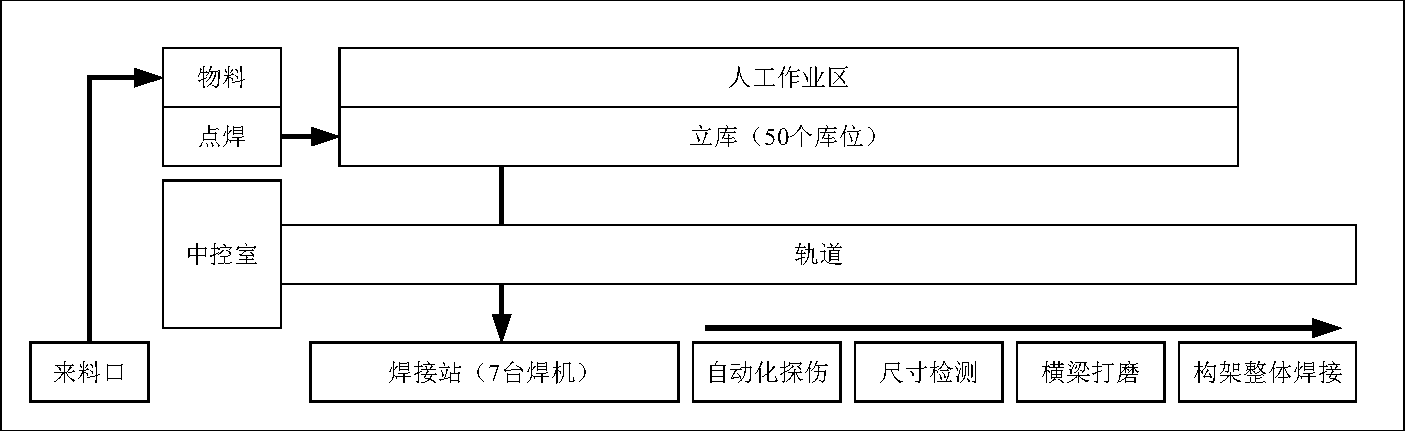
\includegraphics[width=0.98\textwidth, trim=2pt 2pt 2pt 2pt, clip]{assets/GOUJIA_untagged.pdf}
    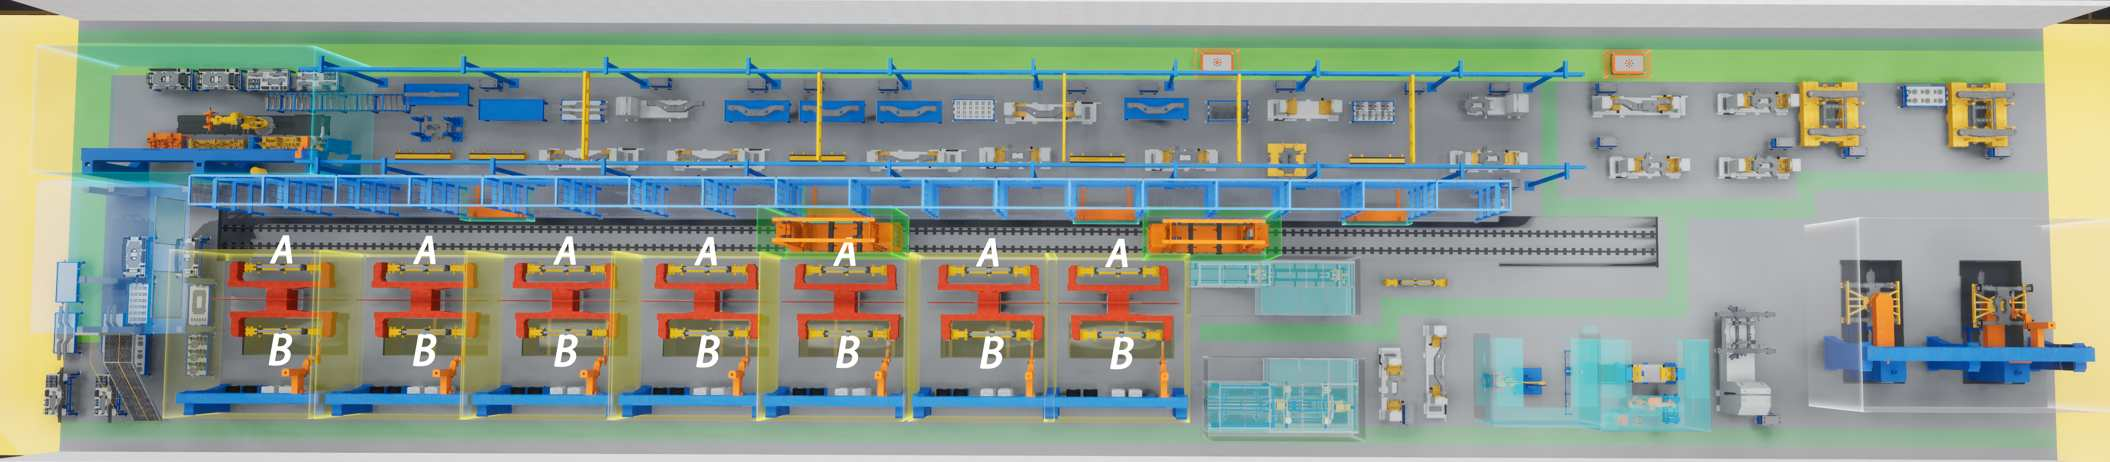
\includegraphics[width=0.96\textwidth]{assets/20260710_120305.jpg}
    \vspace{-2mm}
    \caption{构架焊接智能产线布局示意图}\label{fig:goujia-welding}
    \vspace{-5mm}
  \end{figure}
}

\expandafter\newcommand\csname reportFigure@3\endcsname{
  \begin{figure}[H]
    \centering
    \vspace{-6mm}
    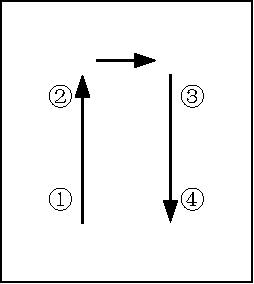
\includegraphics[width=0.25\textwidth, trim=2pt 2pt 2pt 2pt, clip]{assets/U_untagged.pdf}
    \vspace{-9mm}
    \caption{U形生产线示意图}\label{fig:bogie-u-line}
    \vspace{-5mm}
  \end{figure}
}

\expandafter\newcommand\csname reportFigure@4\endcsname{
  \begin{figure}[H]
    \centering
    \vspace{-4mm}
    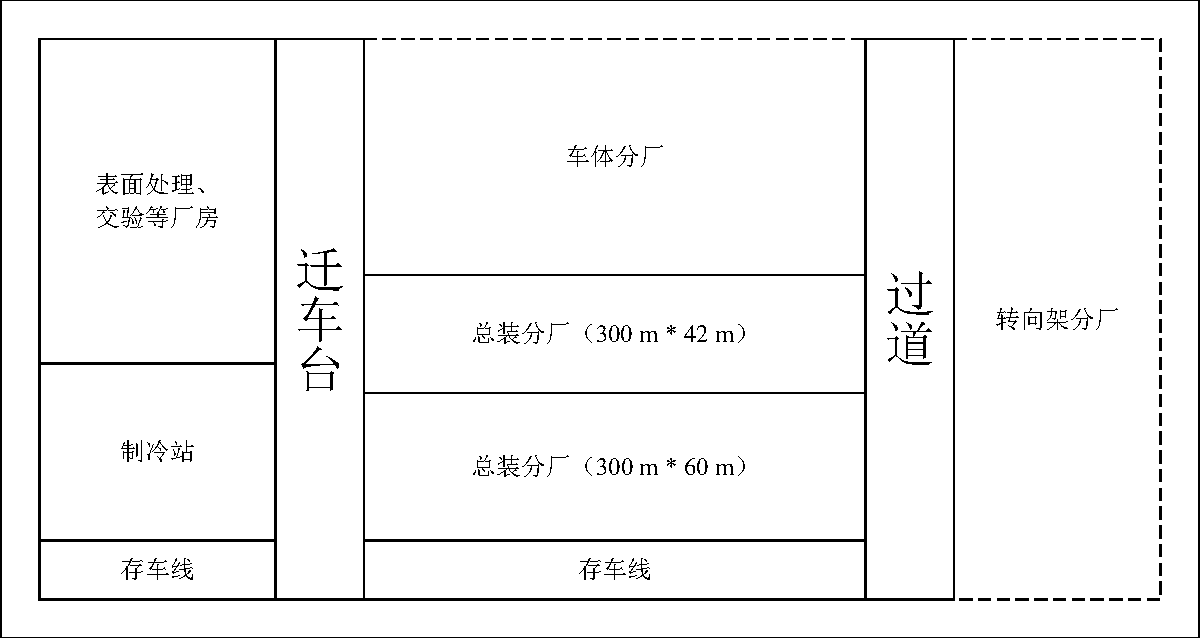
\includegraphics[width=0.8\textwidth, trim=2pt 2pt 2pt 2pt, clip]{assets/MAP_untagged.pdf}
    \vspace{-5mm}
    \caption{总装厂房位置布局（简化）}\label{fig:general-assembly-layout}
    \vspace{-5mm}
  \end{figure}
}

\expandafter\newcommand\csname reportFigure@5\endcsname{
  \begin{figure}[H]
    \centering
    \vspace{-2mm}
    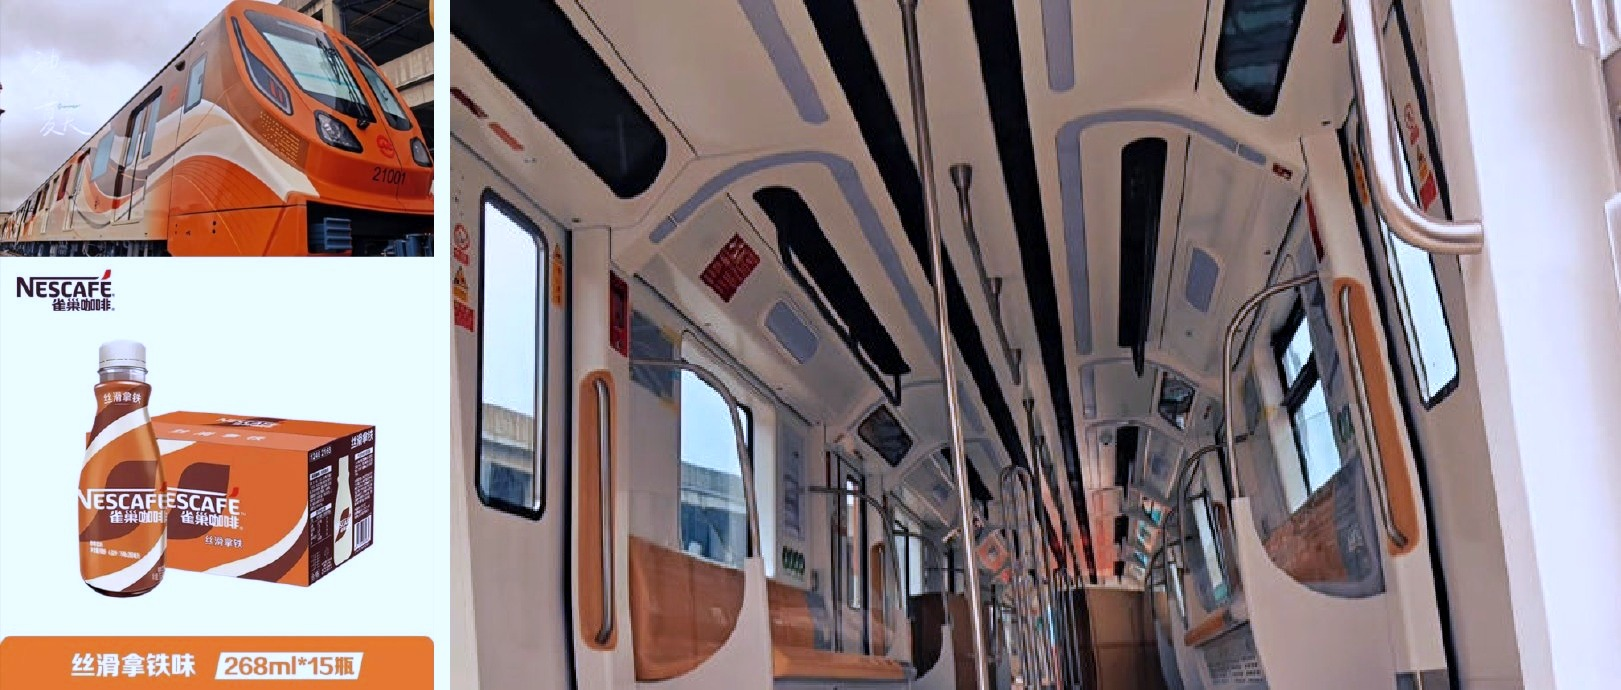
\includegraphics[width=0.98\textwidth]{assets/L21-corrected.jpg}
    \vspace{-2mm}
    \caption{上海地铁21号线列车外观与内装示意}\label{fig:l21-train}
    \vspace{-5mm}
  \end{figure}
}

\expandafter\newcommand\csname reportFigure@8\endcsname{
  \begin{figure}[H]
    \centering
    \vspace{-3mm}
    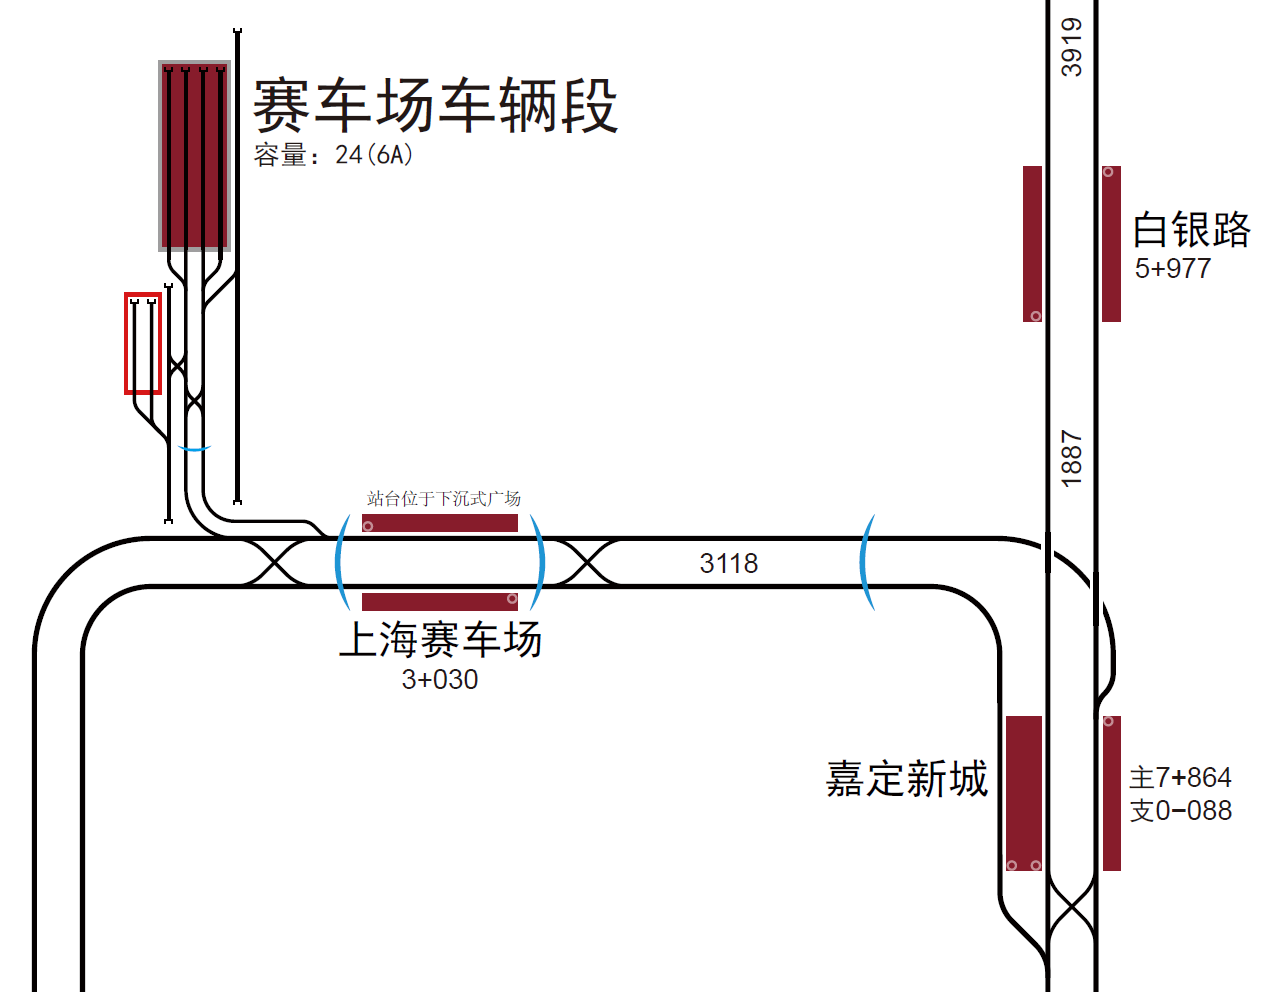
\includegraphics[width=0.48\textwidth]{assets/day6.png}
    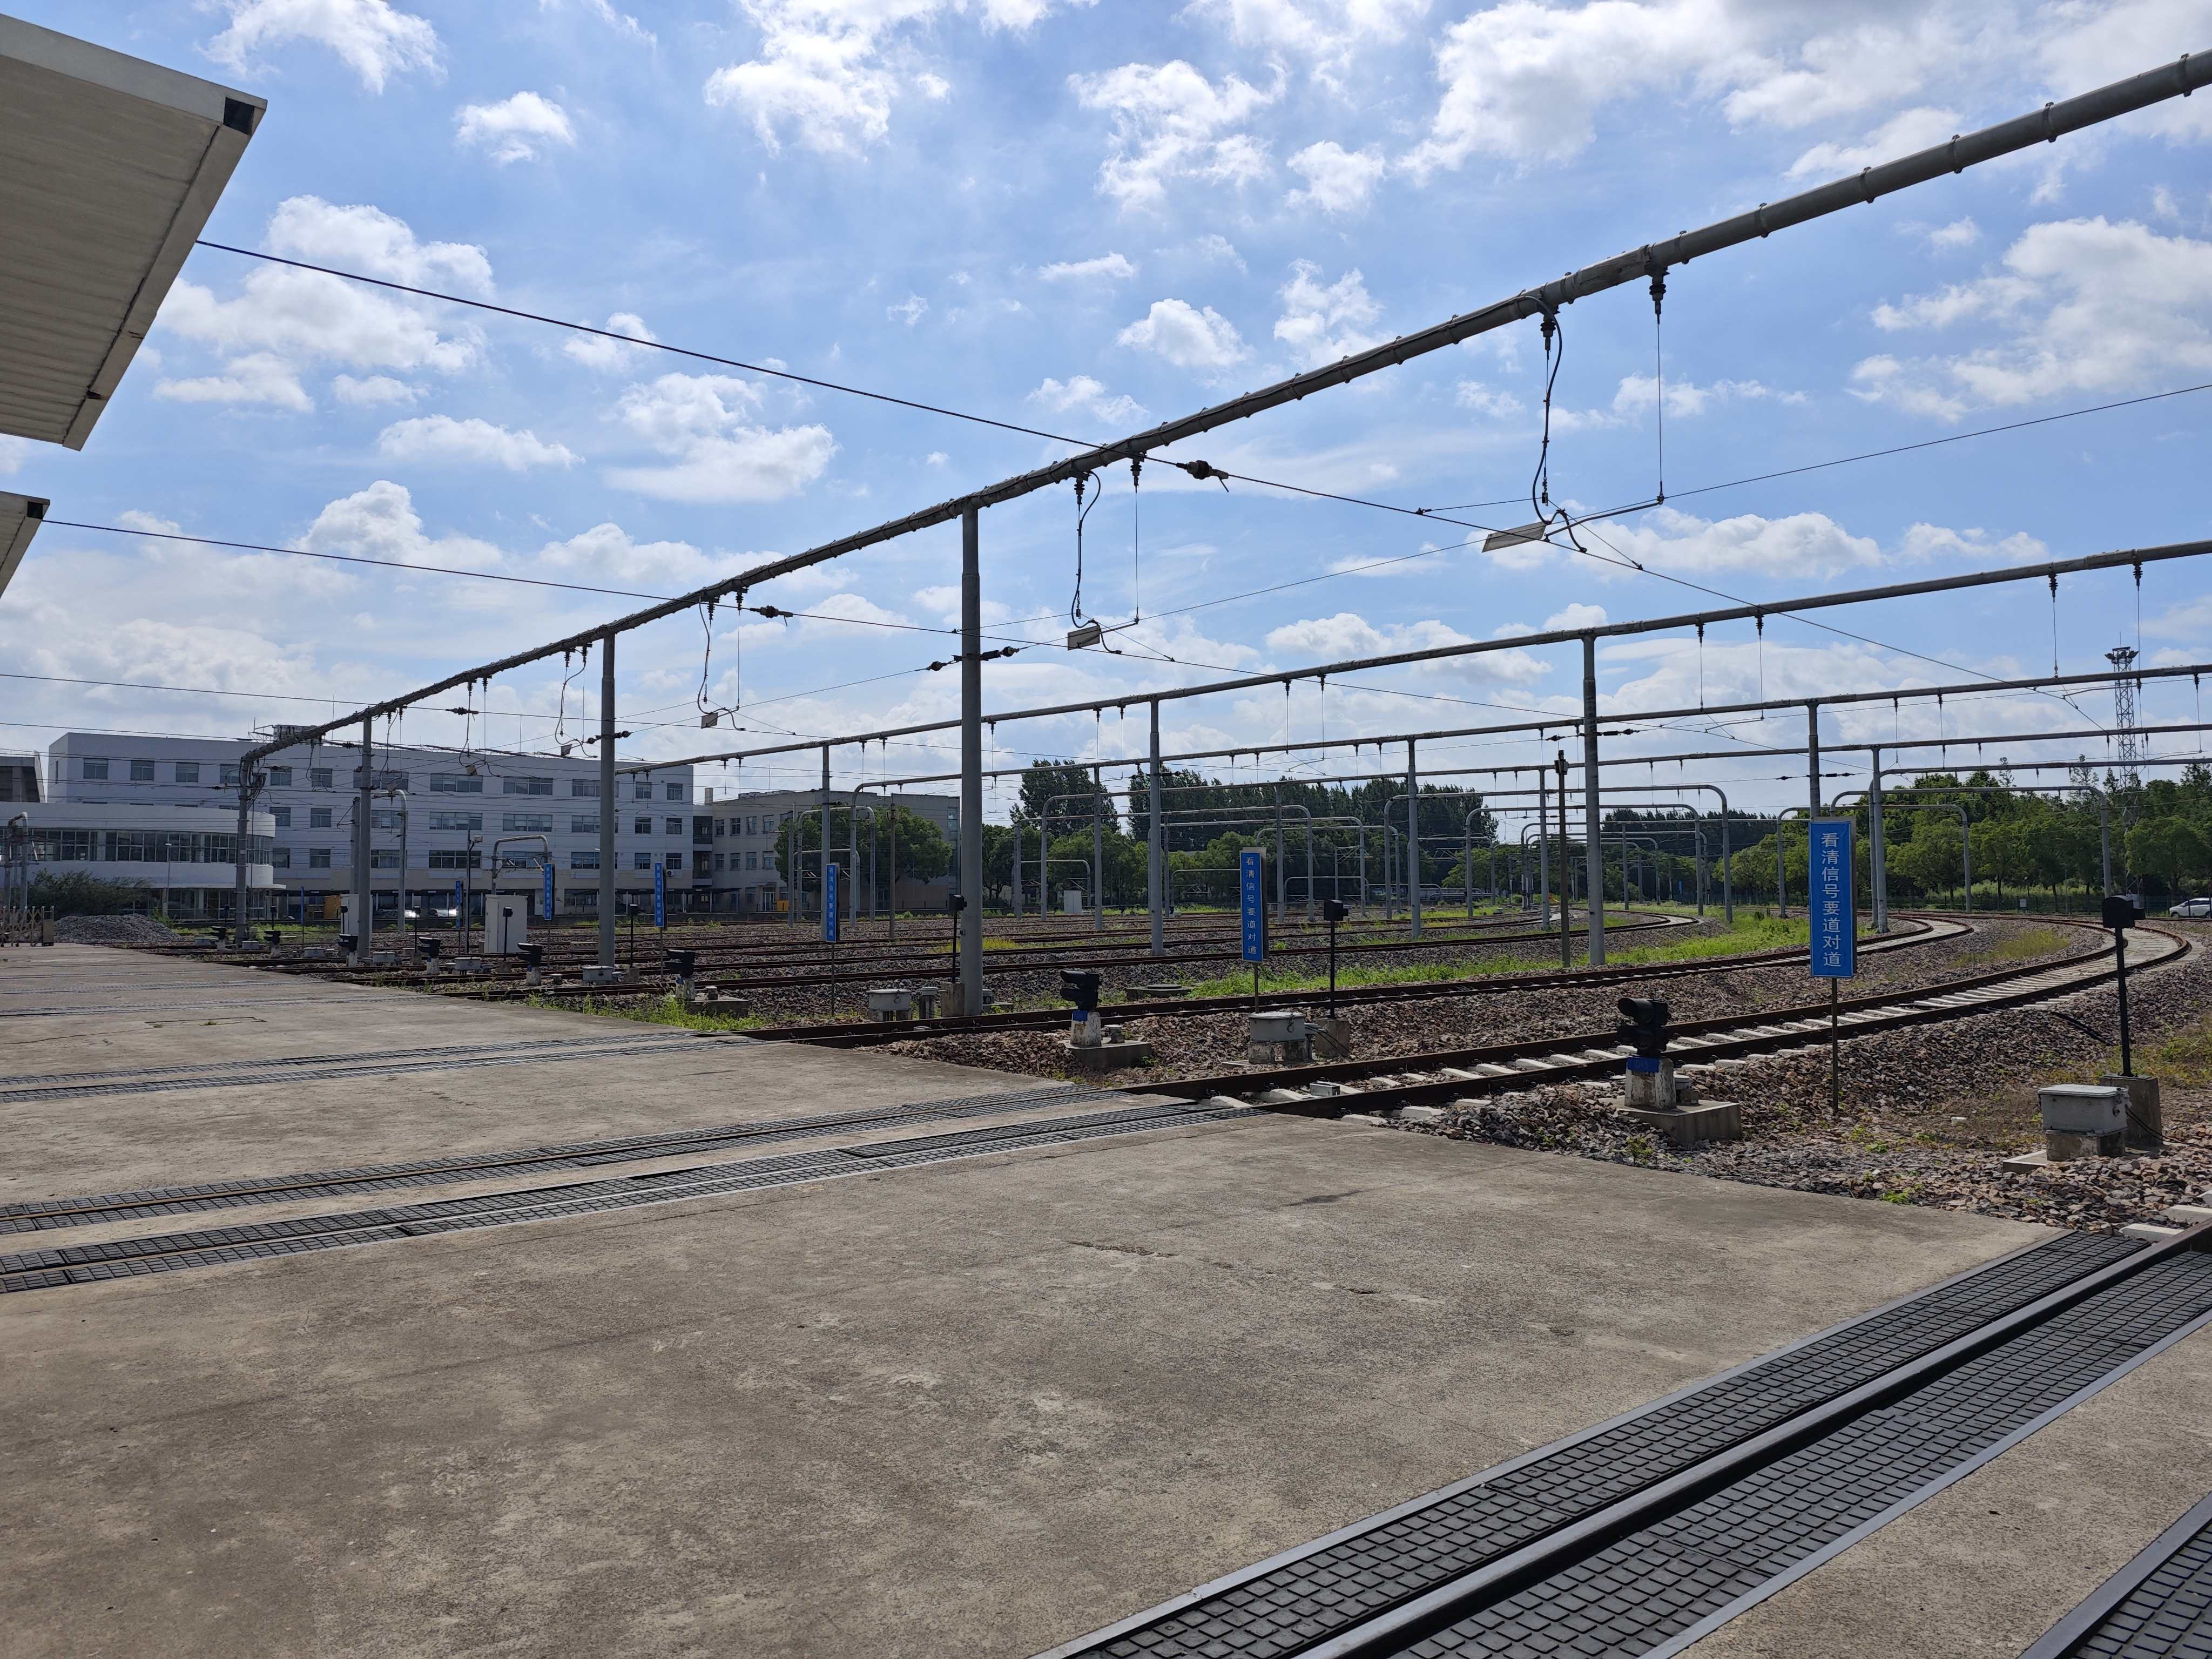
\includegraphics[width=0.5\textwidth]{assets/20260716_233131.jpg}
    \vspace{-2mm}
    \caption{上海赛车场车辆段位置与概况}\label{fig:saichang-maintenance-base}
    \vspace{-5mm}
  \end{figure}
}

\expandafter\newcommand\csname reportInlineFigure@9\endcsname{
  \centering
  \vspace{0pt}
  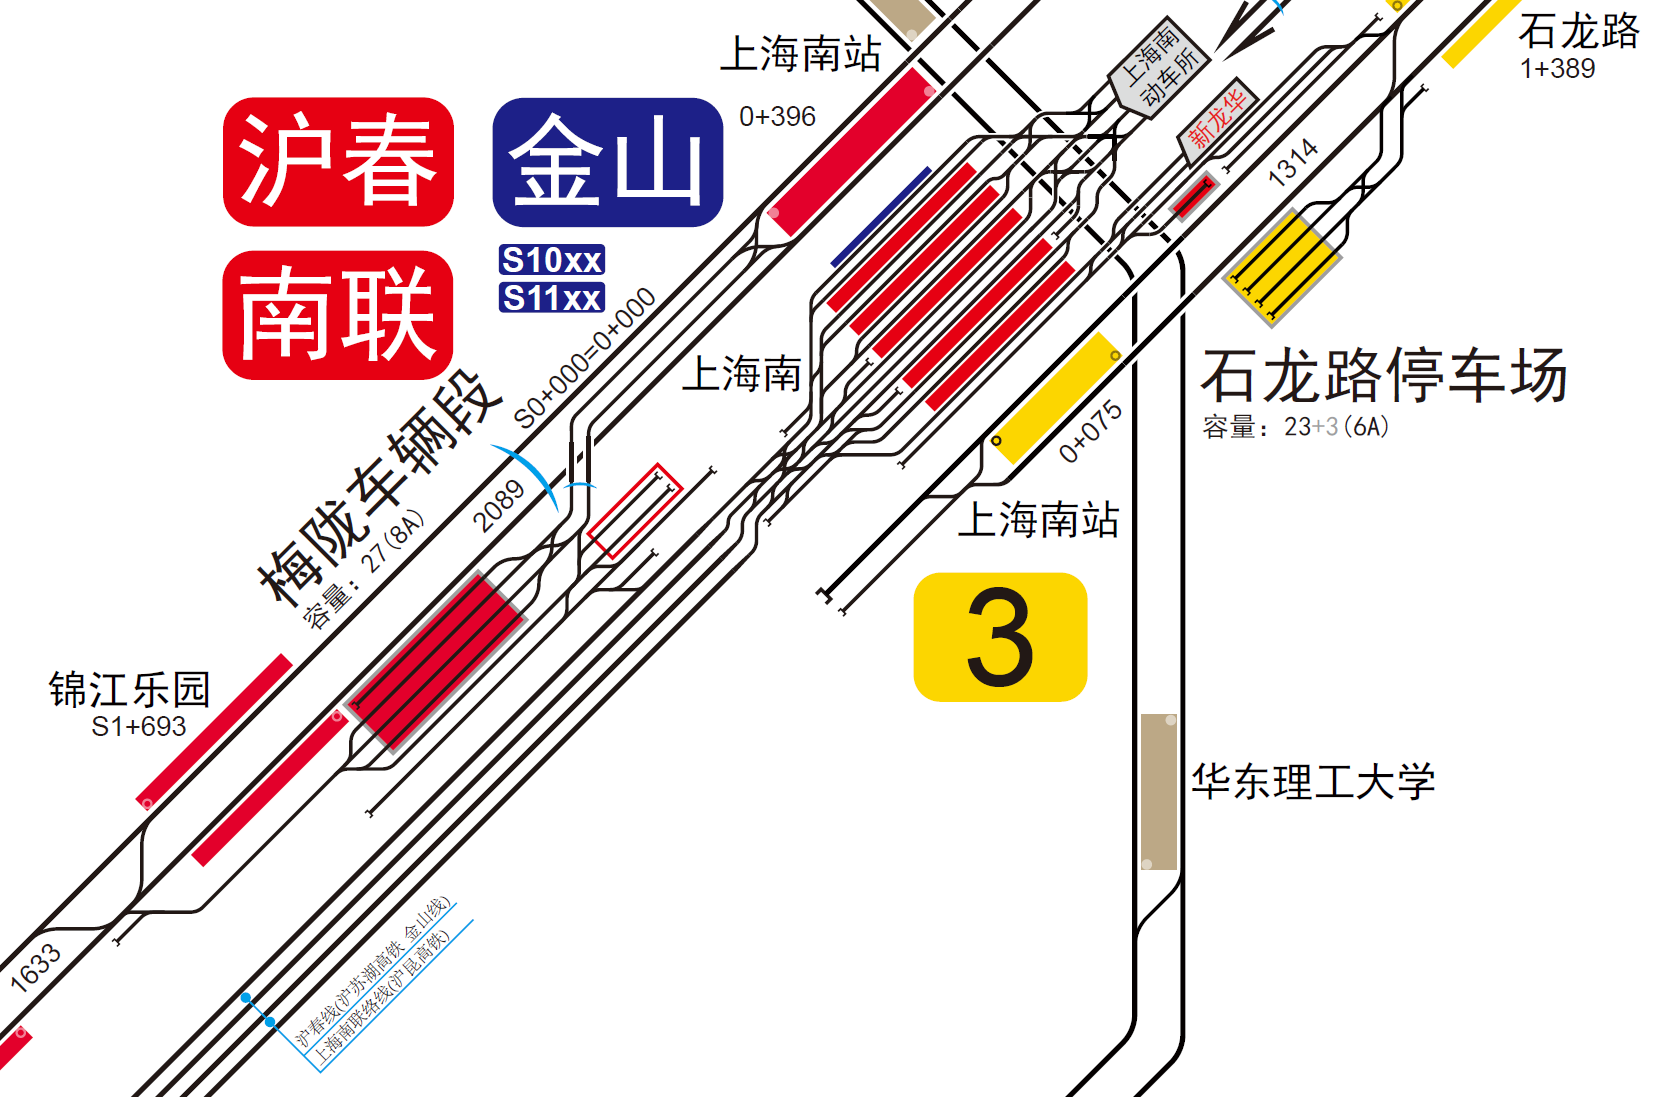
\includegraphics[width=\linewidth]{assets/day7.png}
  \vspace{-7mm}
  \captionof{figure}{梅陇基地位置}\label{fig:meilong-base}
}

\expandafter\newcommand\csname reportFigure@10\endcsname{
  \begin{figure}[H]
    \centering
    \vspace{-3mm}
    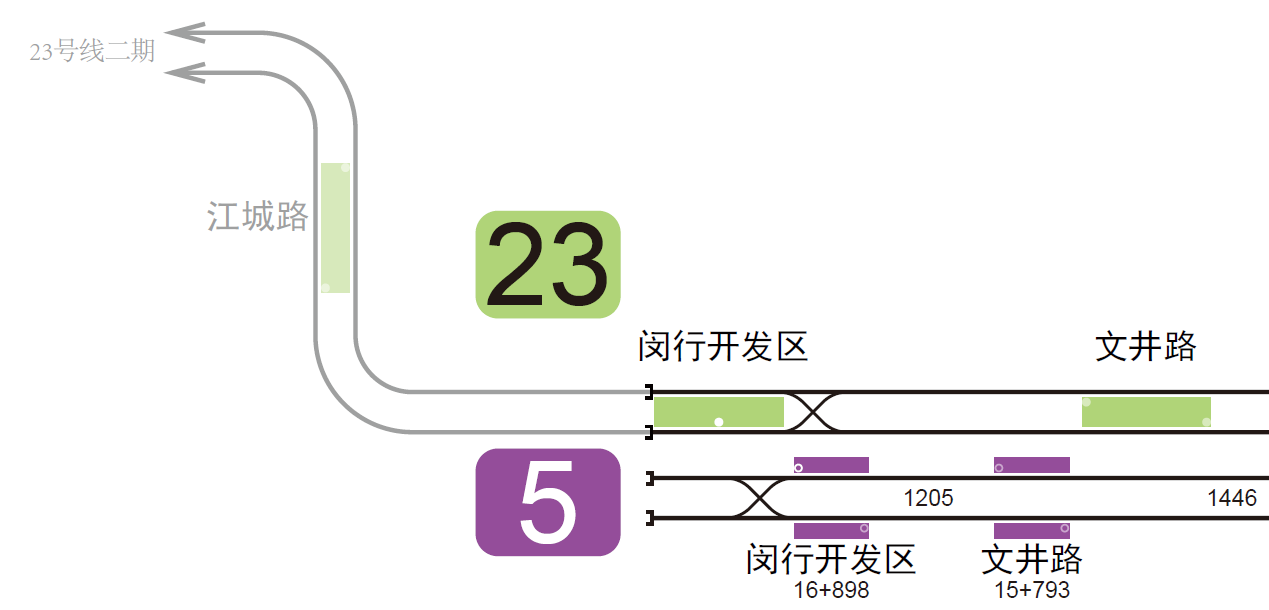
\includegraphics[width=0.6\textwidth]{assets/day8.png}
    \vspace{-2mm}
    \caption{上海阿尔斯通（中车长客）公司位置}\label{fig:satee-position}
    \vspace{-5mm}
  \end{figure}
}

\expandafter\newcommand\csname reportFigure@11\endcsname{
  \begin{figure}[H]
    \centering
    \vspace{-3mm}
    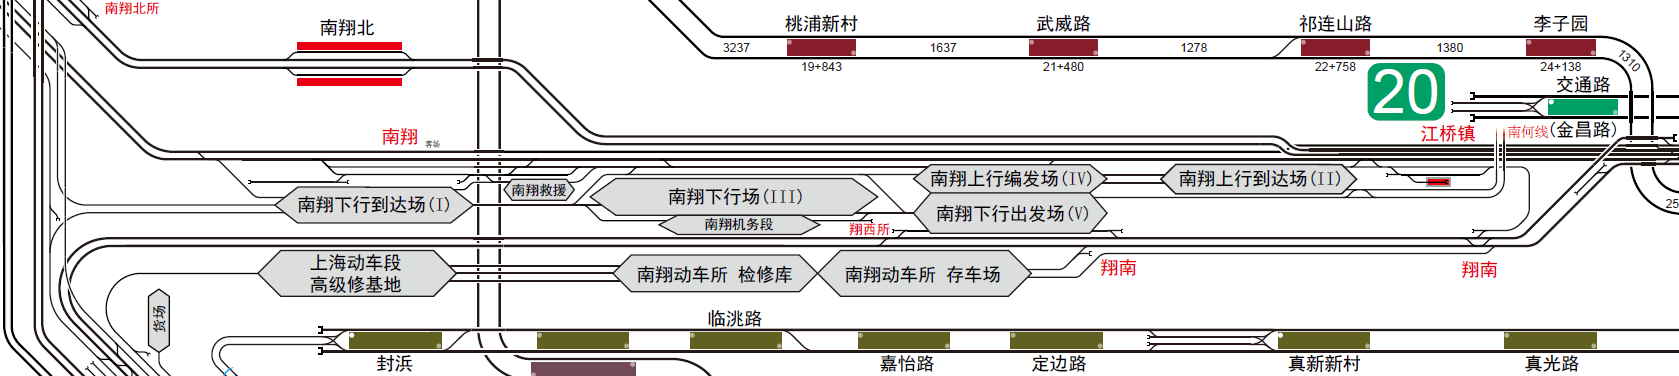
\includegraphics[width=0.98\textwidth]{assets/day9.png}
    \vspace{-2mm}
    \caption{上海动车段动车组高级修场位置}\label{fig:shanghai-emu-depot}
    \vspace{-5mm}
  \end{figure}
}

\expandafter\newcommand\csname reportFigure@12\endcsname{
  \begin{figure}[H]
    \centering
    \vspace{-2.5mm}
    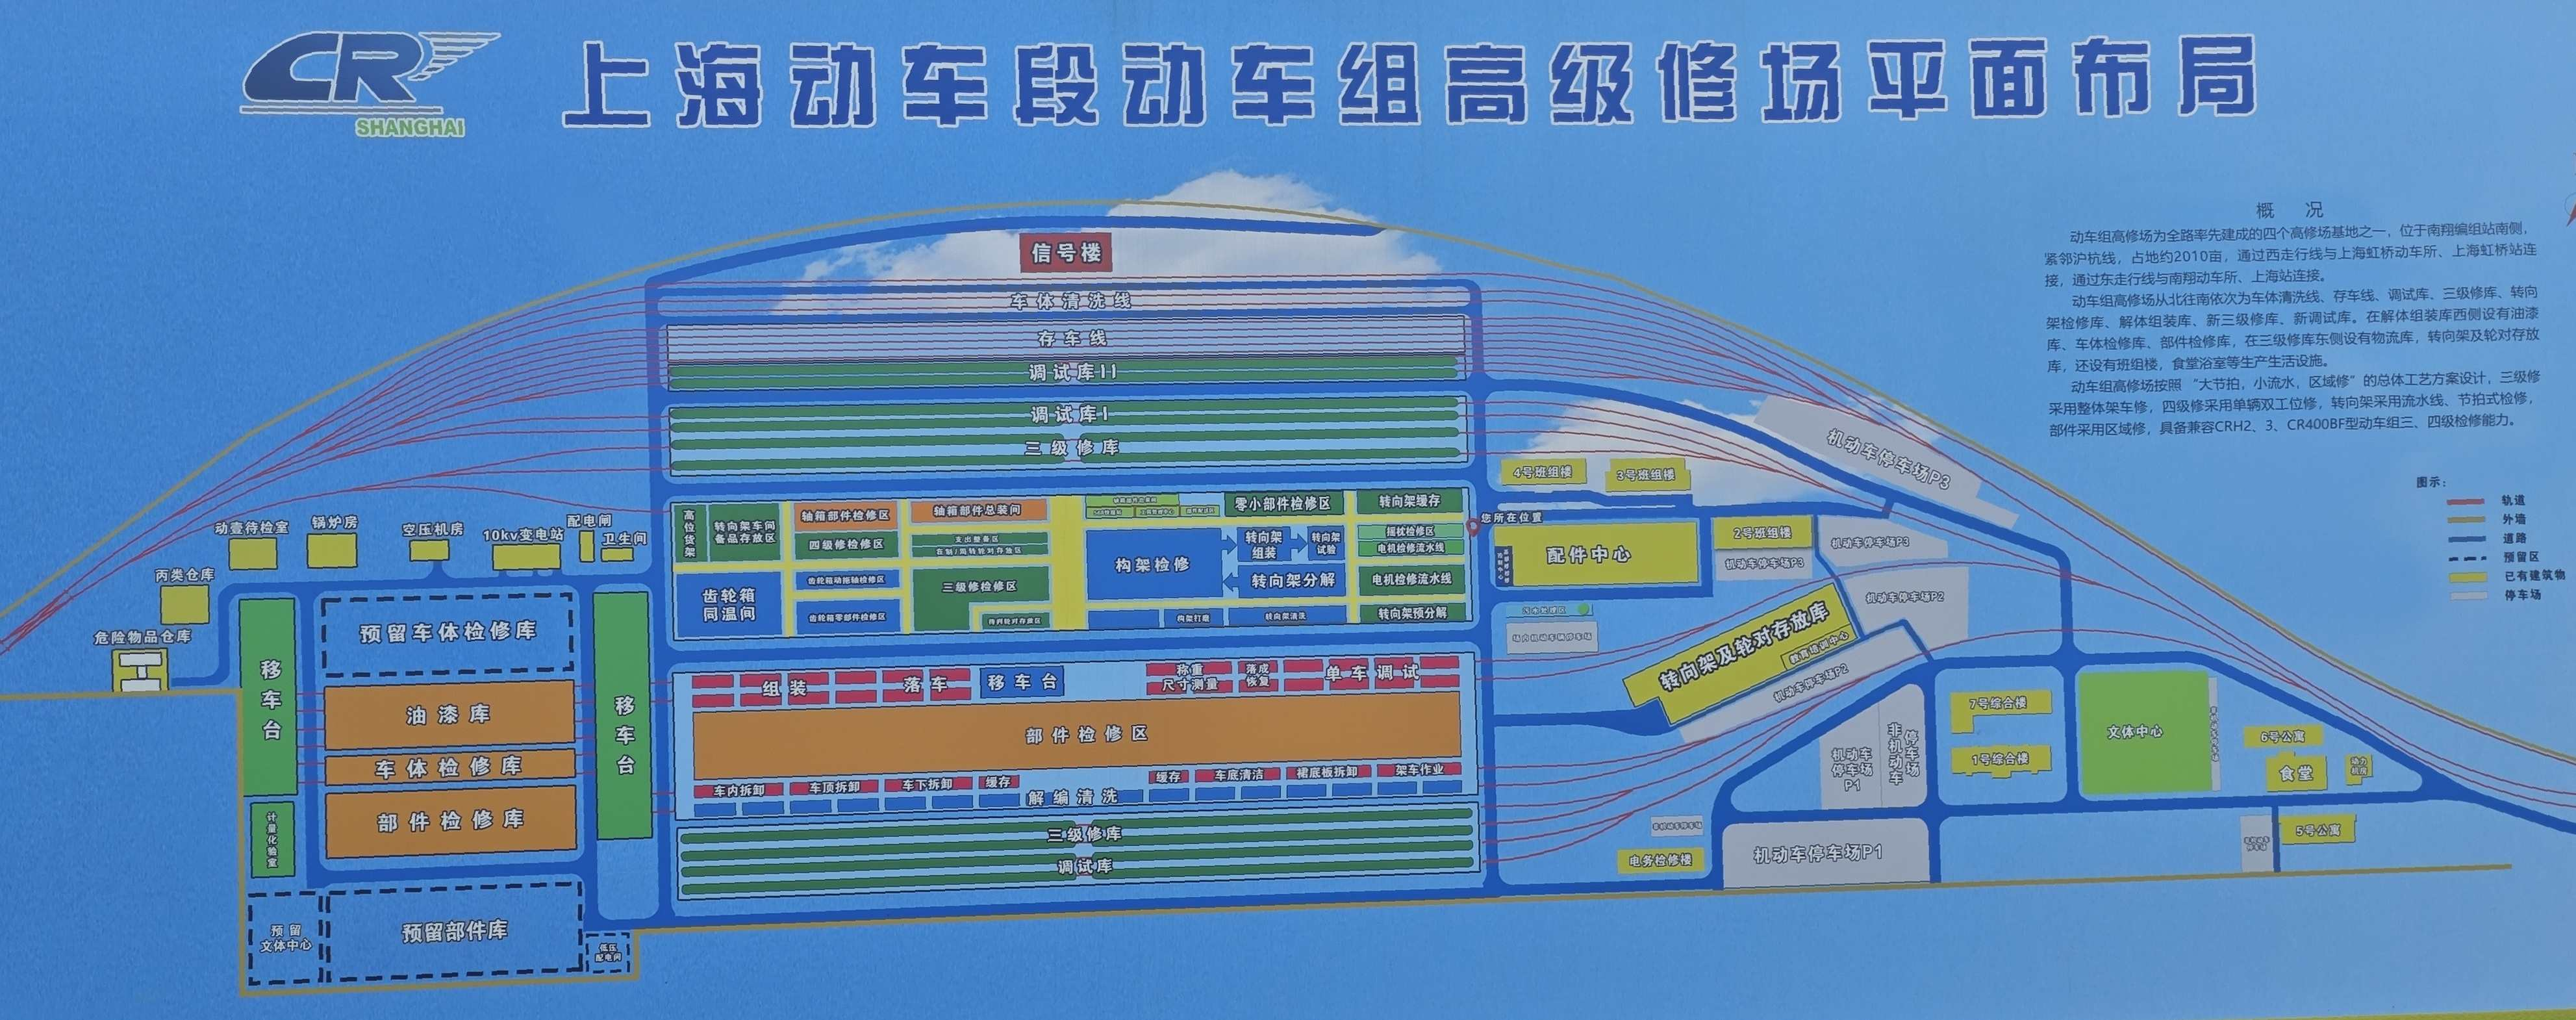
\includegraphics[width=0.98\textwidth]{assets/20260718_211523.jpg}
    \vspace{-2.5mm}
    \caption{上海动车段动车组高级修场内部布局图}\label{fig:emu-overhaul-yard-layout}
    \vspace{-5mm}
  \end{figure}
}

\expandafter\newcommand\csname reportFigure@13\endcsname{
  \begin{figure}[H]
    \centering
    \vspace{-1mm}
    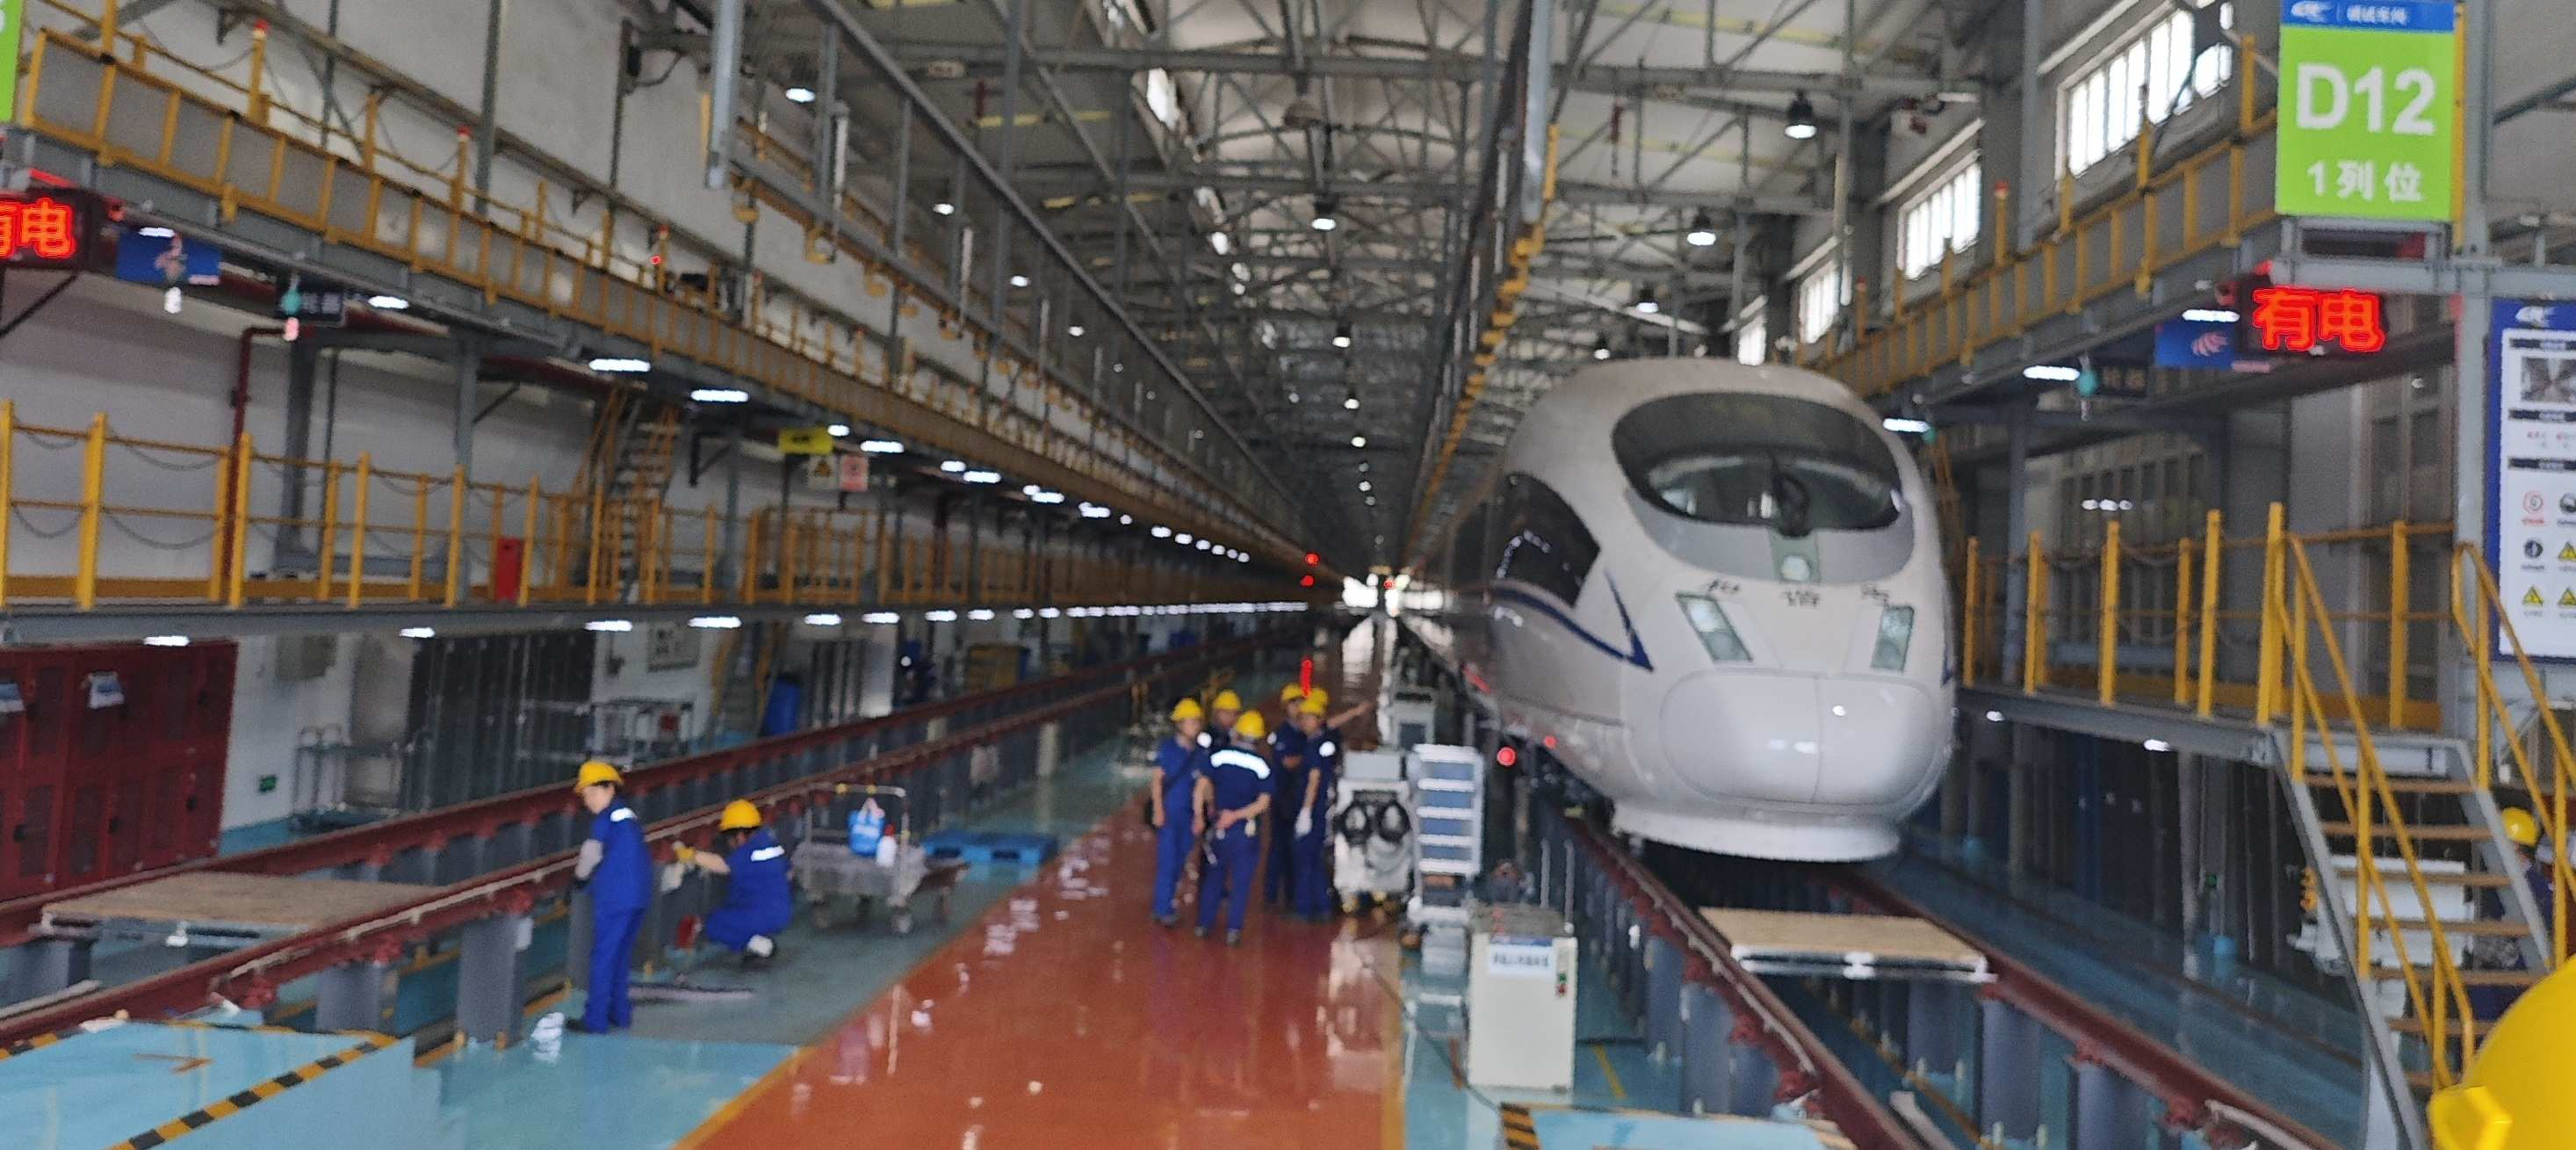
\includegraphics[width=0.8\textwidth]{assets/20260718_212836.jpg}
    \vspace{-2.5mm}
    \caption{正在检修的CRH380BL-3545列车}\label{fig:crh380bl-3545-overhaul}
    \vspace{-5mm}
  \end{figure}
}

\expandafter\newcommand\csname reportFigure@14\endcsname{
  \begin{figure}[H]
    \centering
    \vspace{-1mm}
    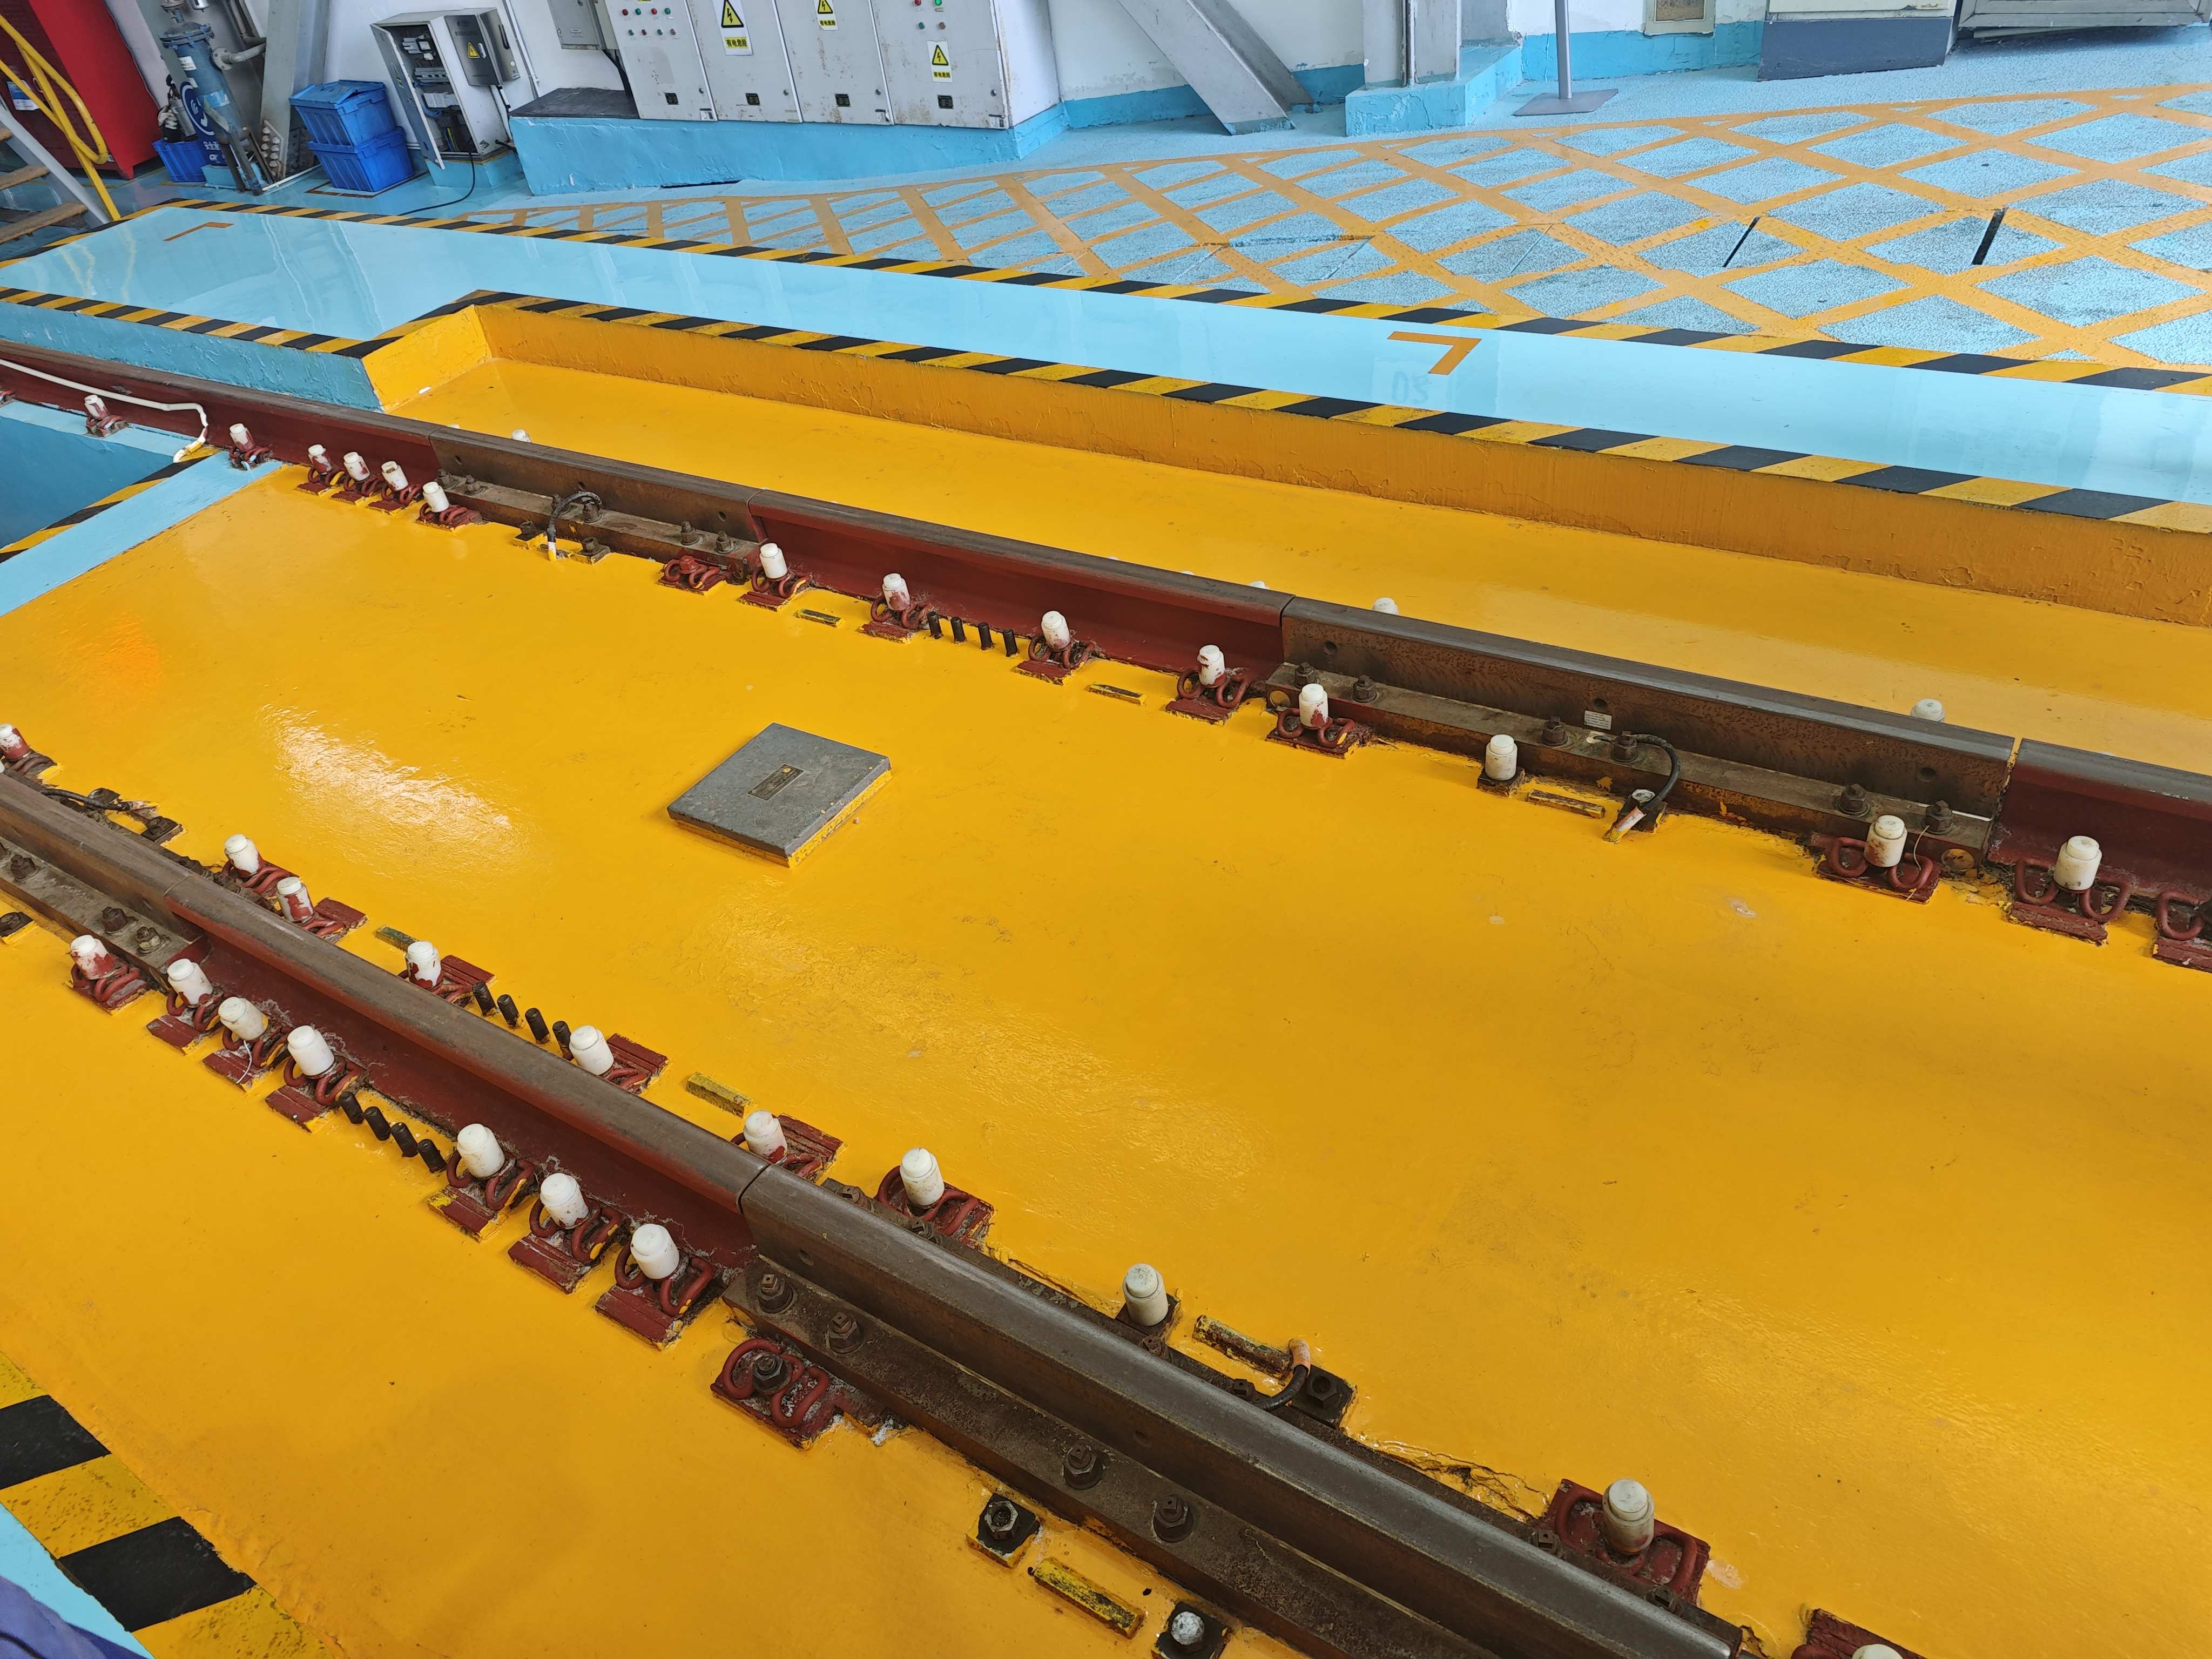
\includegraphics[width=0.32\textwidth]{assets/20260718_215423.jpg}
    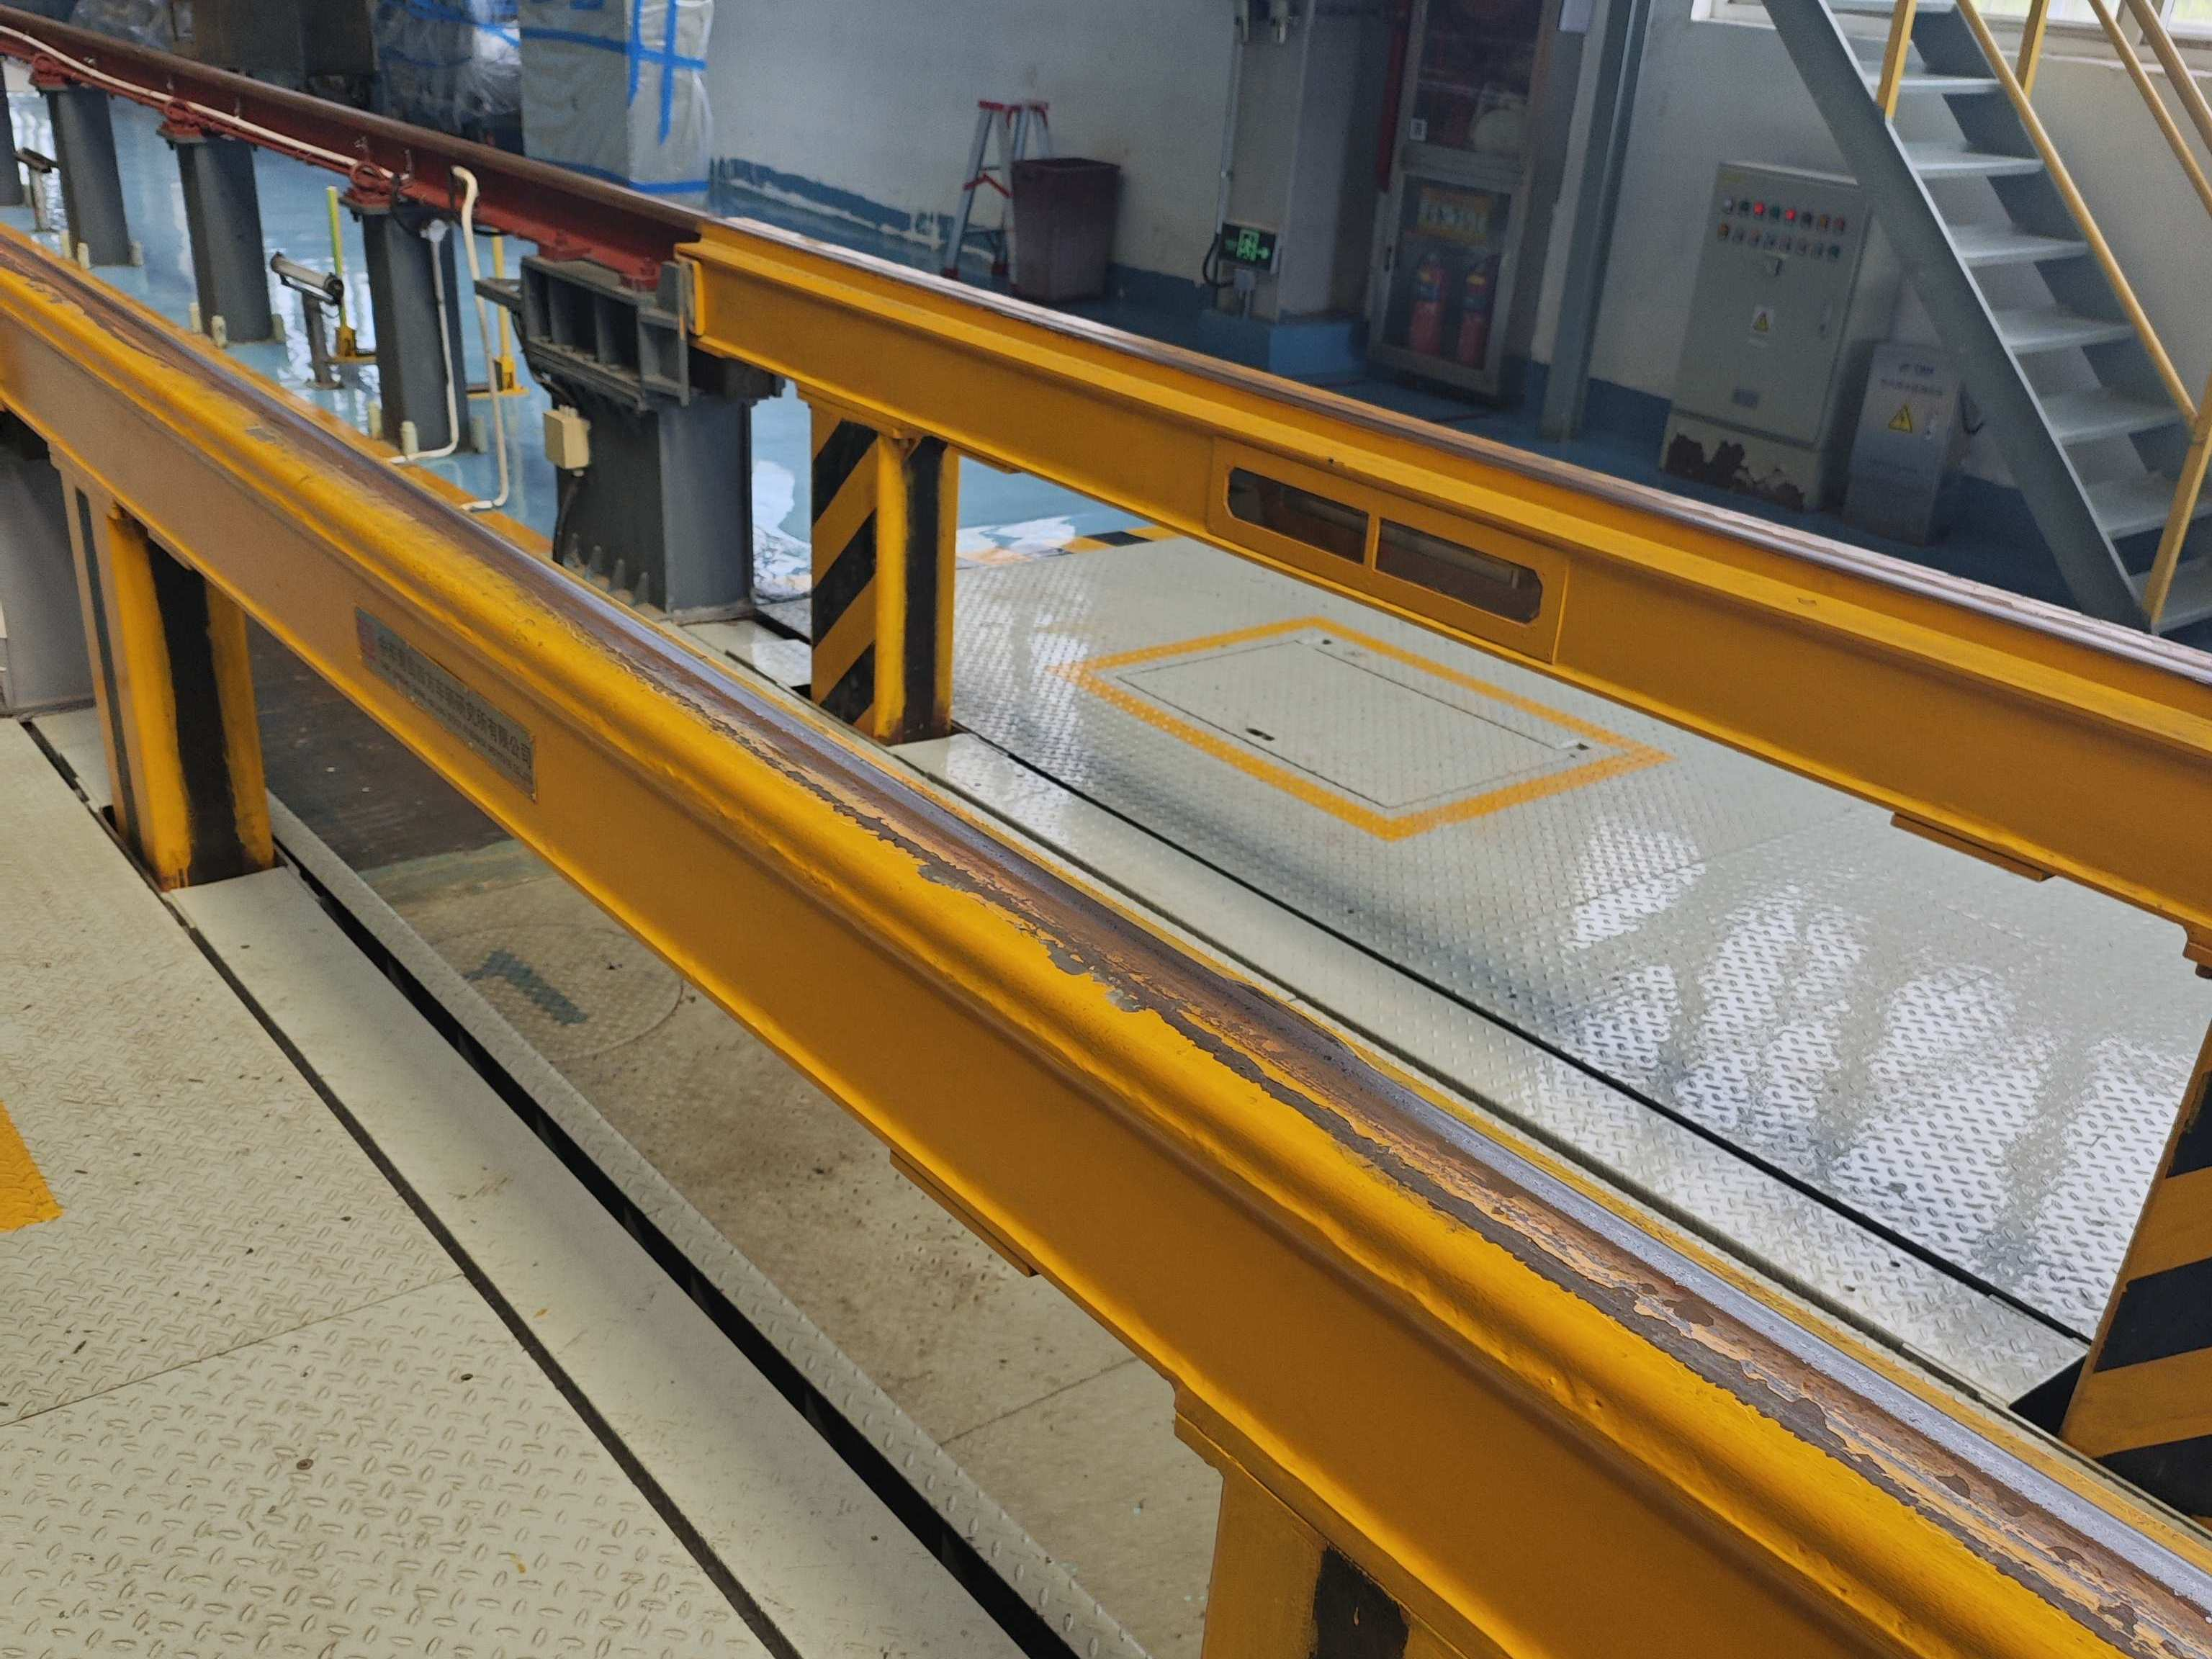
\includegraphics[width=0.32\textwidth]{assets/20260718_215429.jpg}
    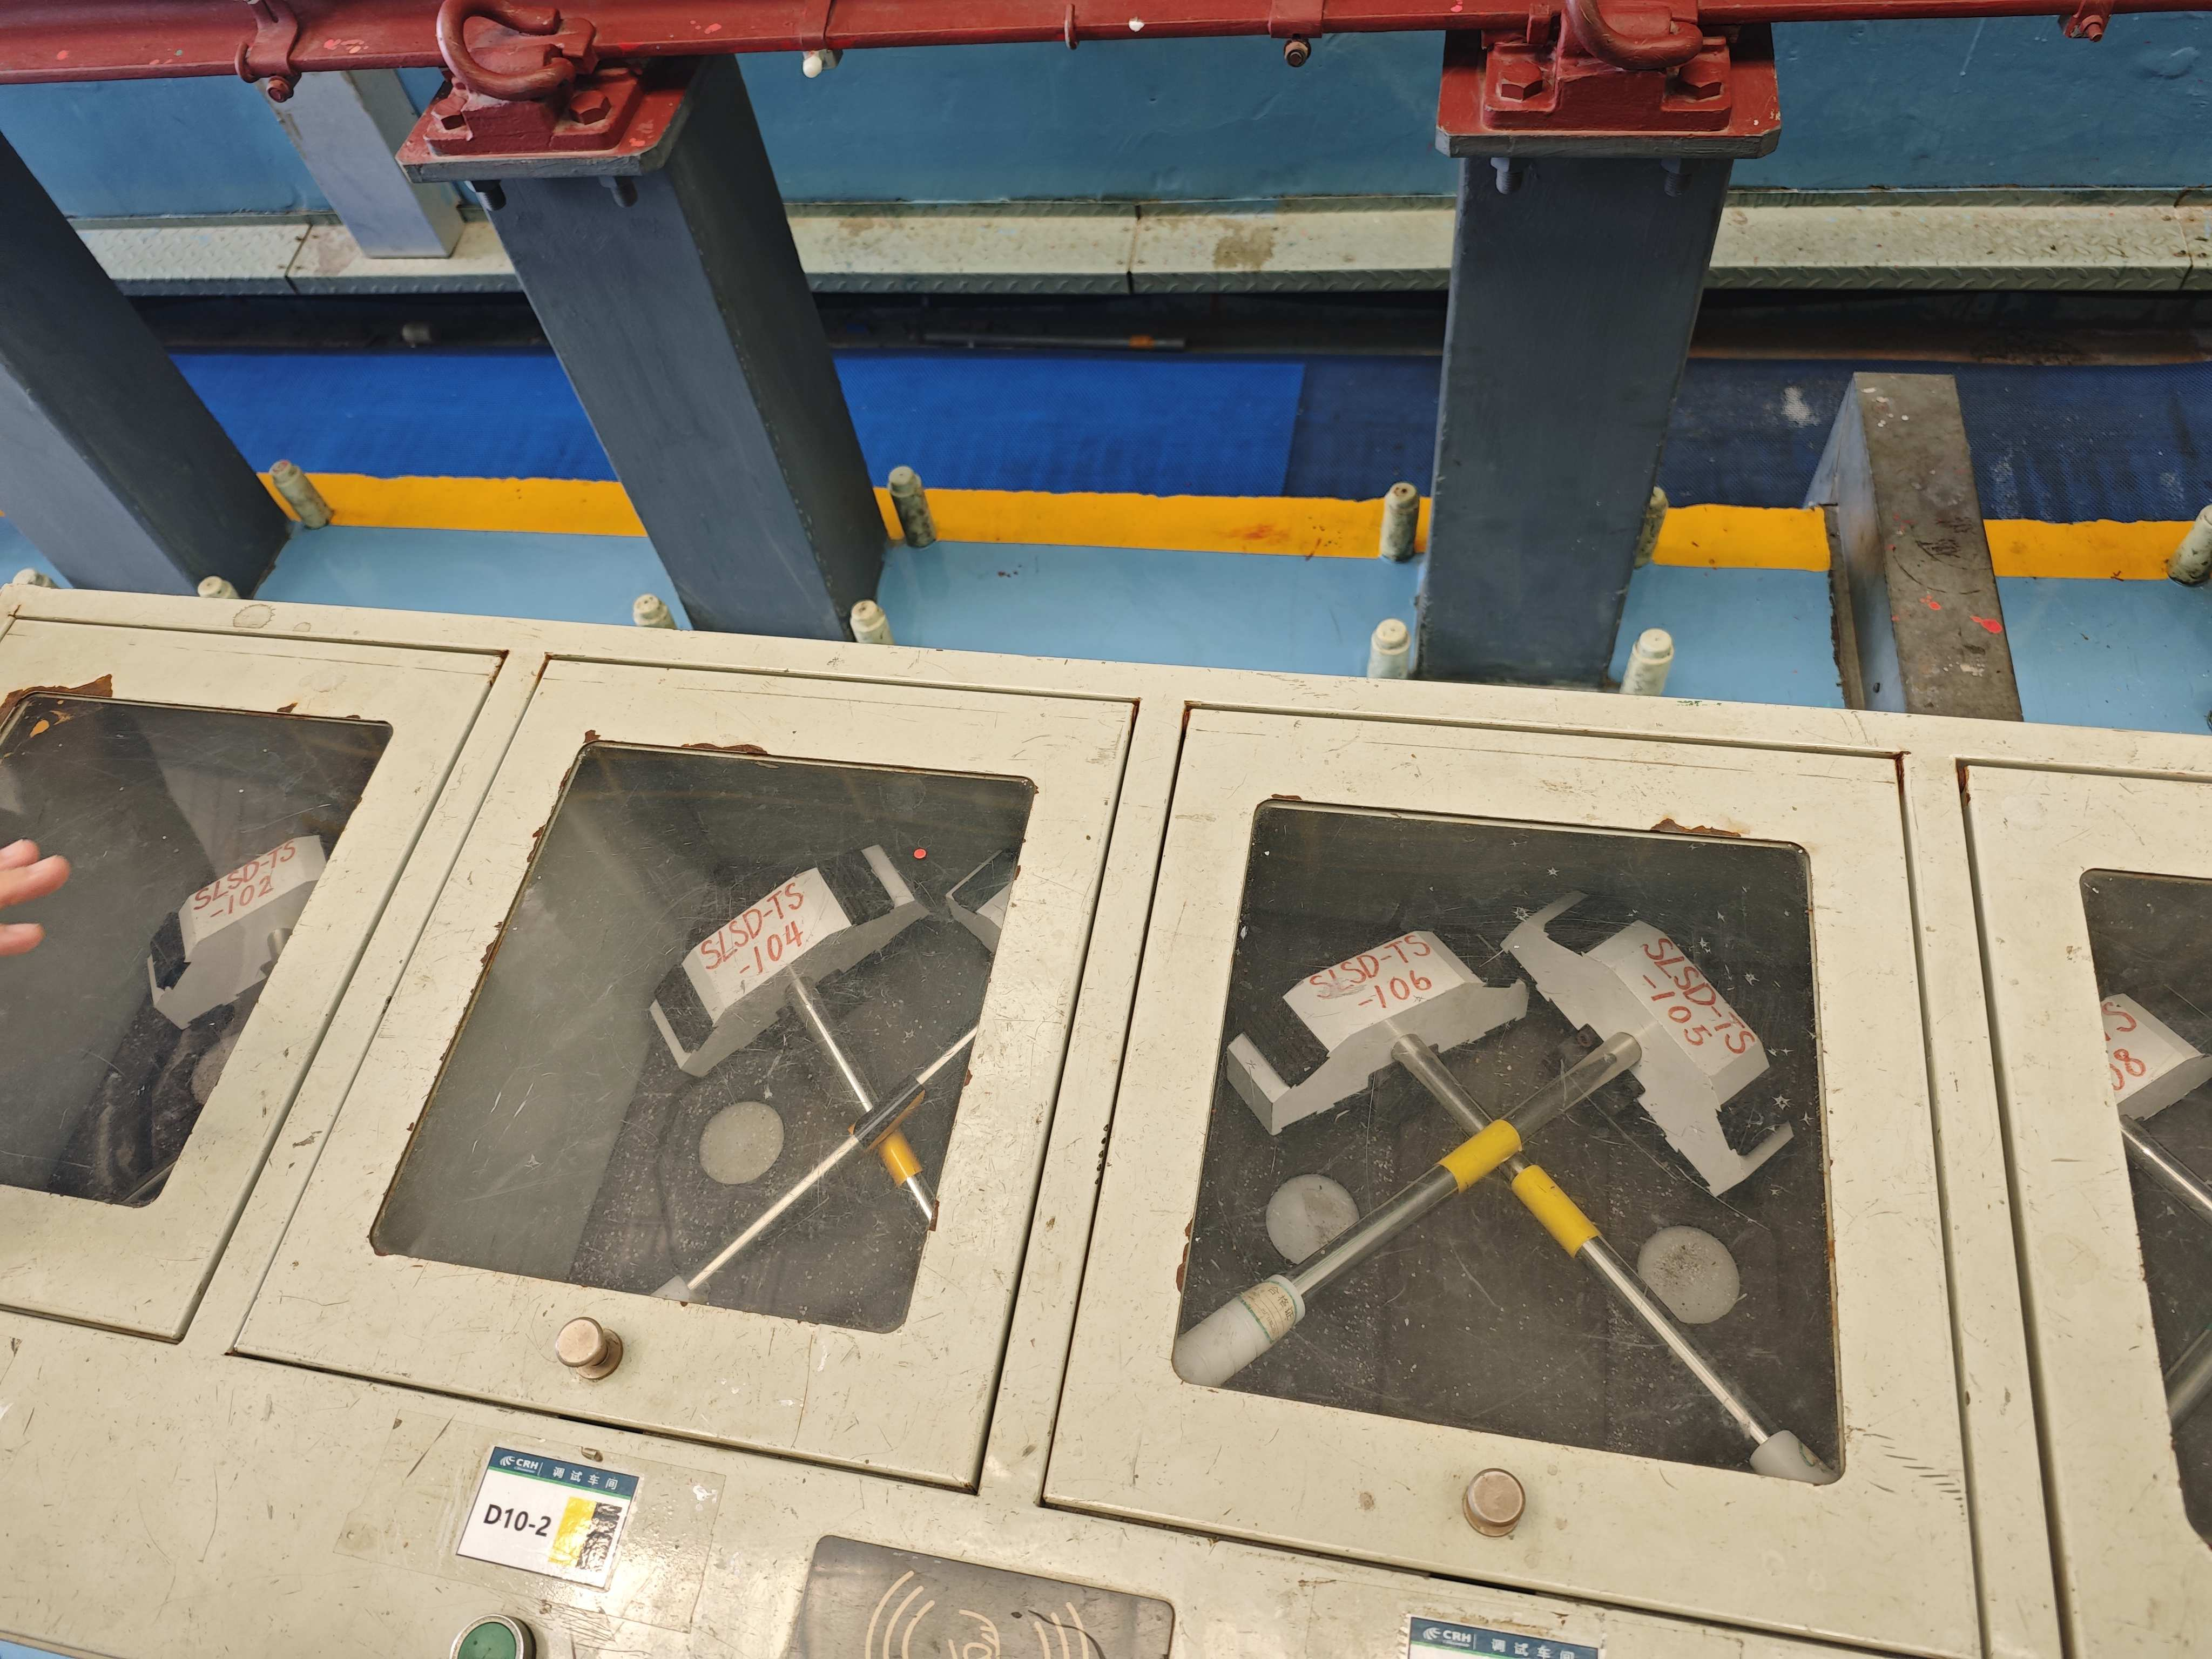
\includegraphics[width=0.32\textwidth]{assets/20260718_215456.jpg}
    \vspace{-2.5mm}
    \caption{部分检修用设备}\label{fig:overhaul-equipment}
    \vspace{-5mm}
  \end{figure}
}

\expandafter\newcommand\csname reportFigure@15\endcsname{
  \begin{figure}[H]
    \centering
    \vspace{-1mm}
    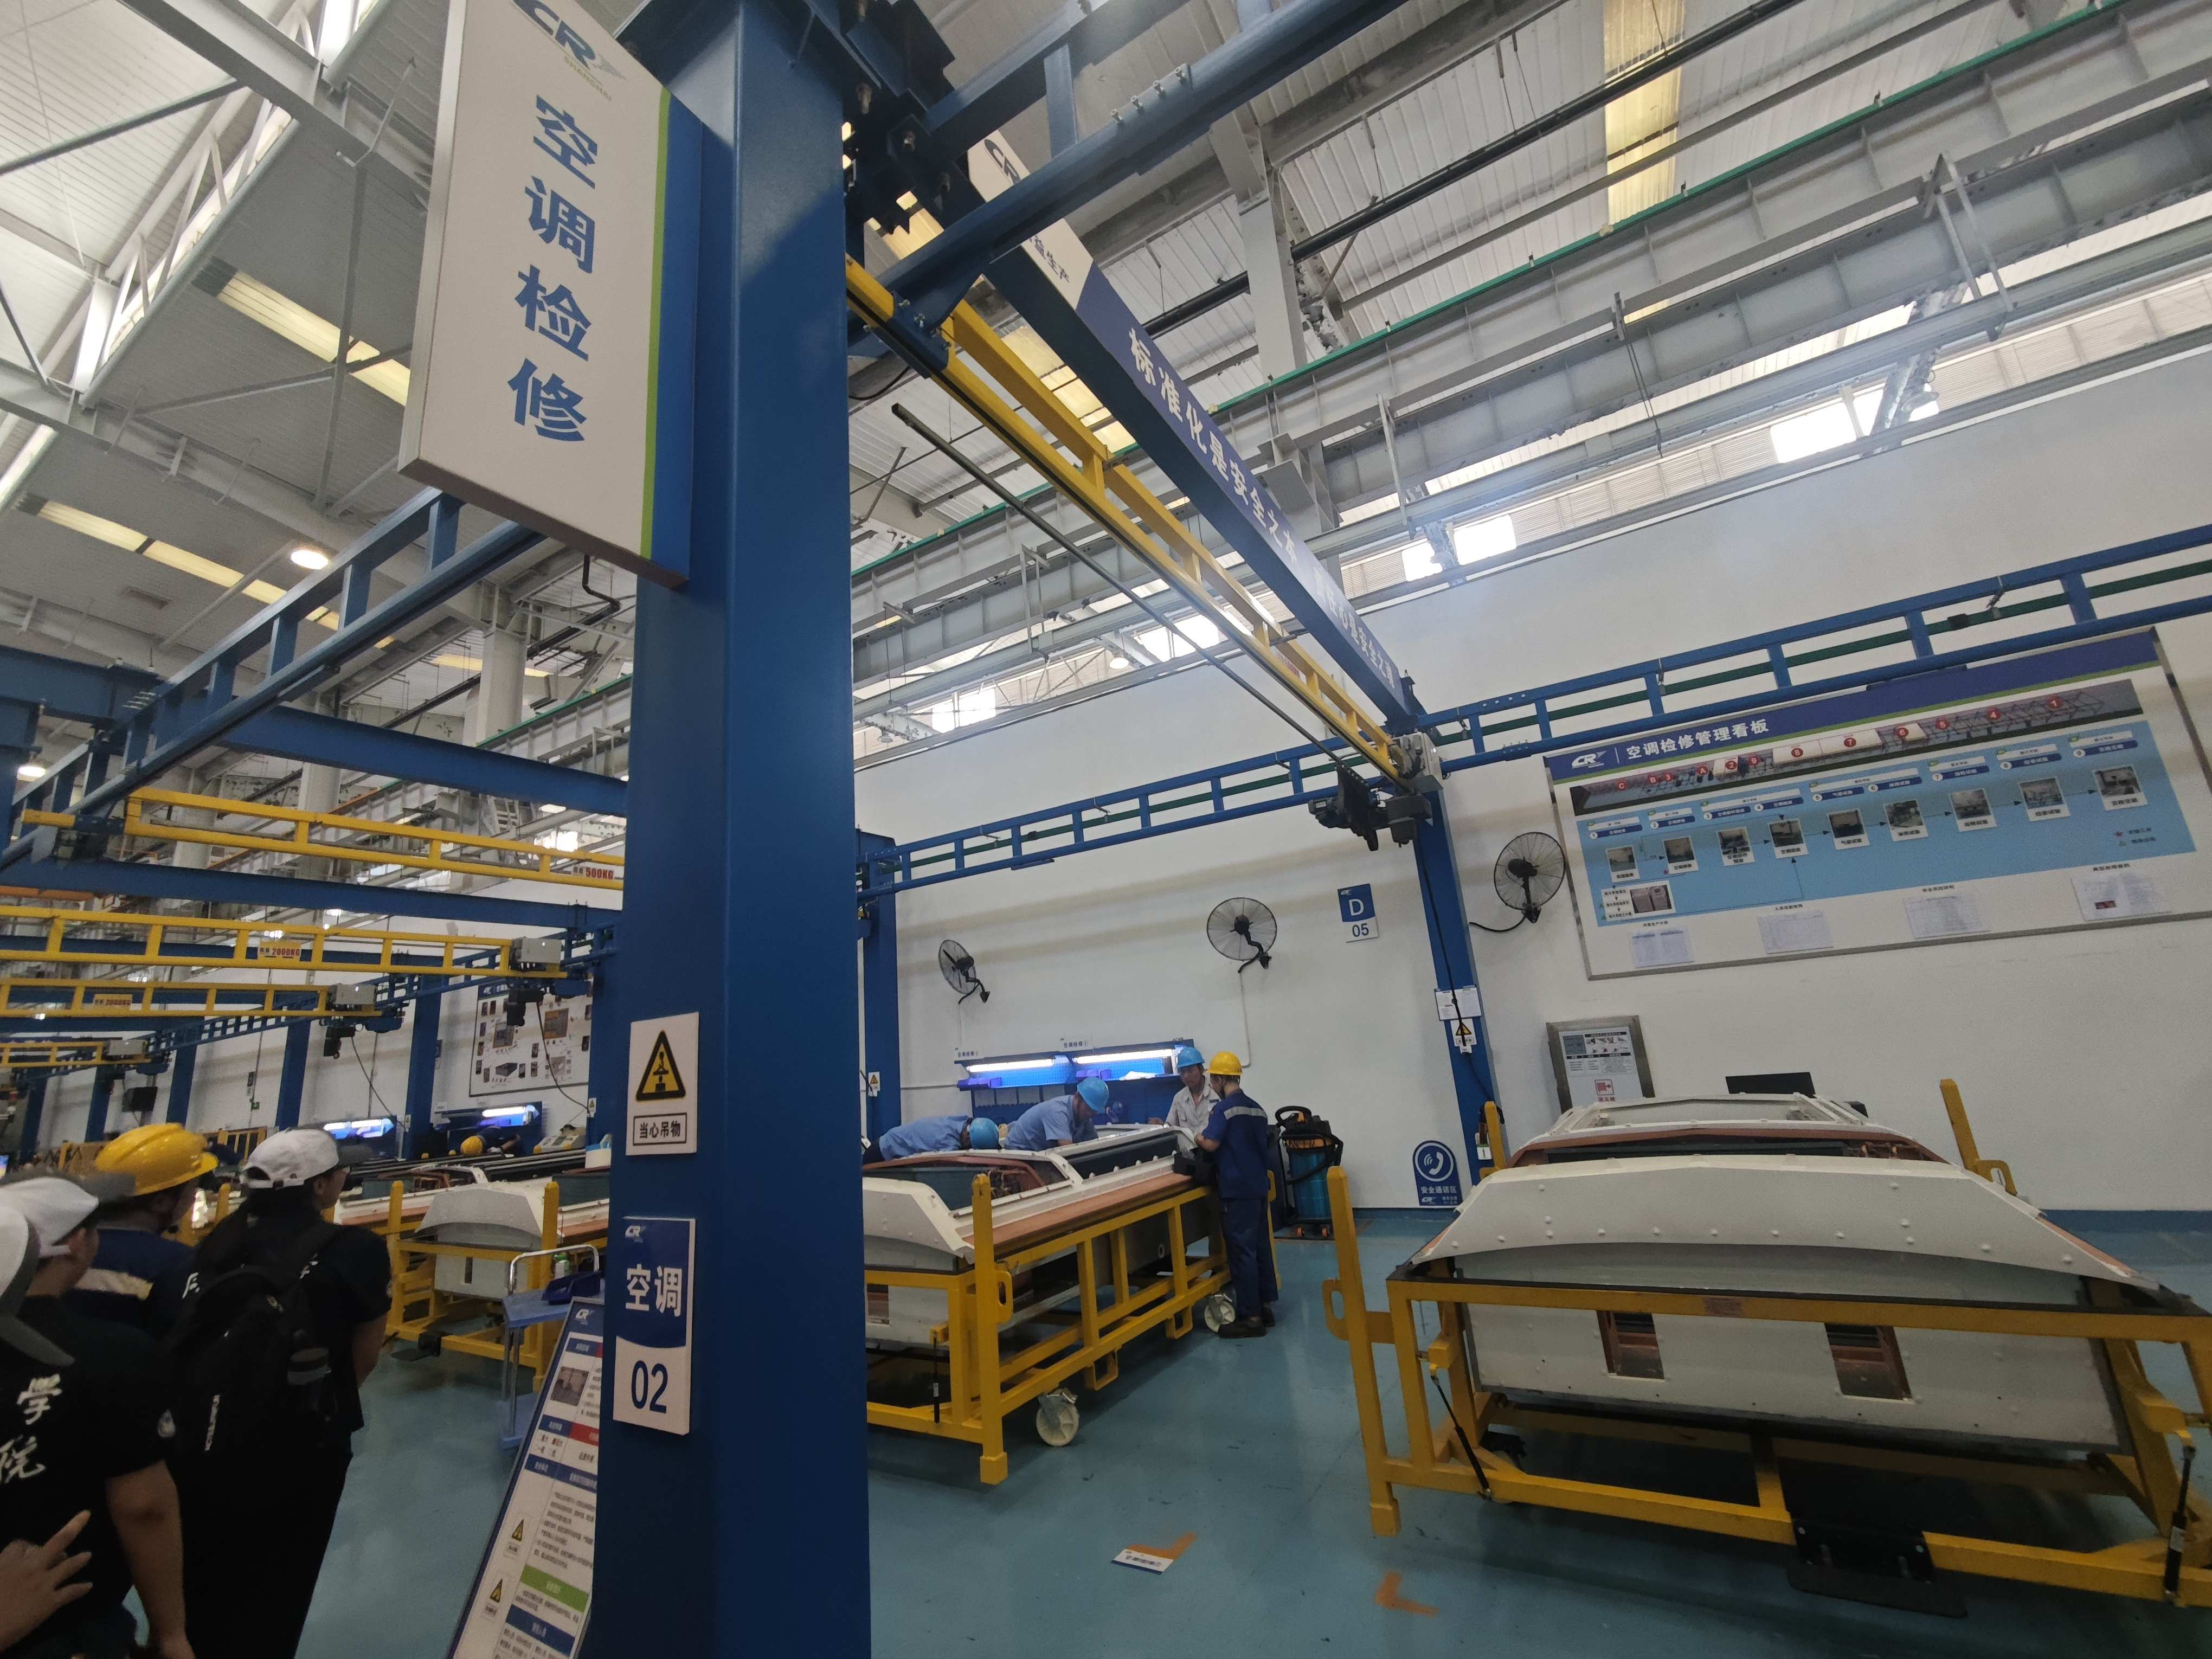
\includegraphics[width=0.32\textwidth]{assets/20260718_234723.jpg}
    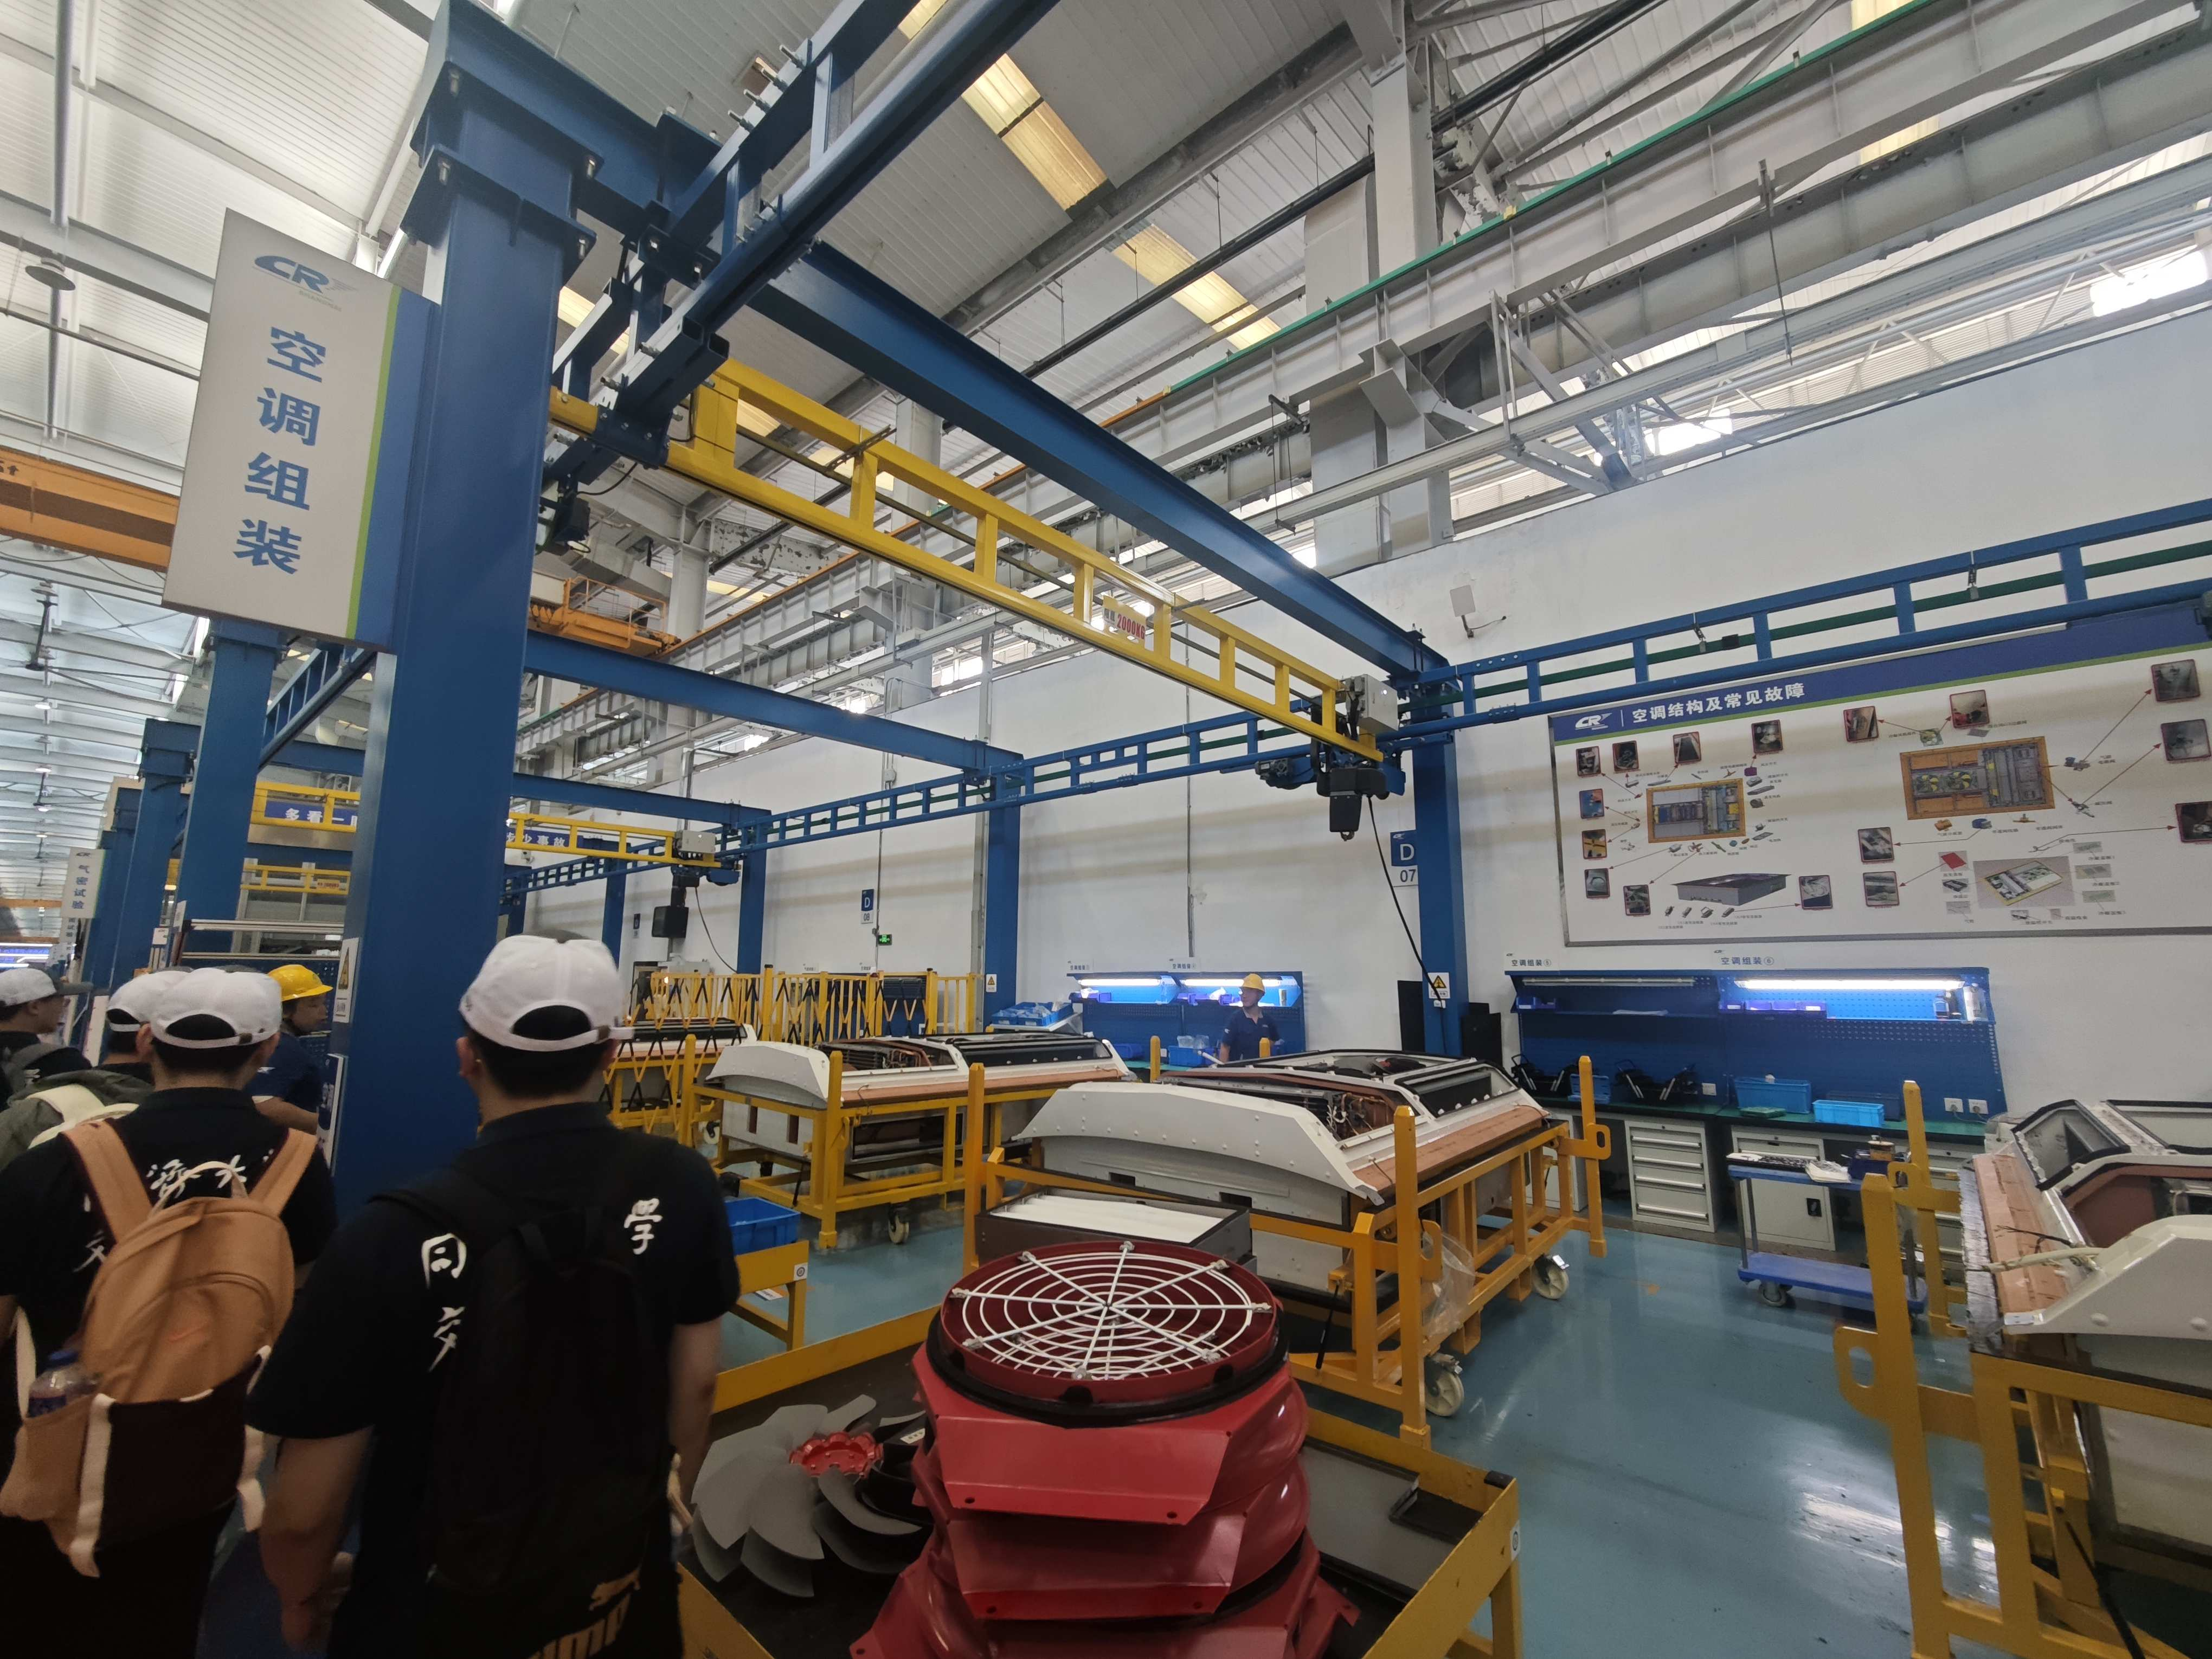
\includegraphics[width=0.32\textwidth]{assets/20260718_234735.jpg}
    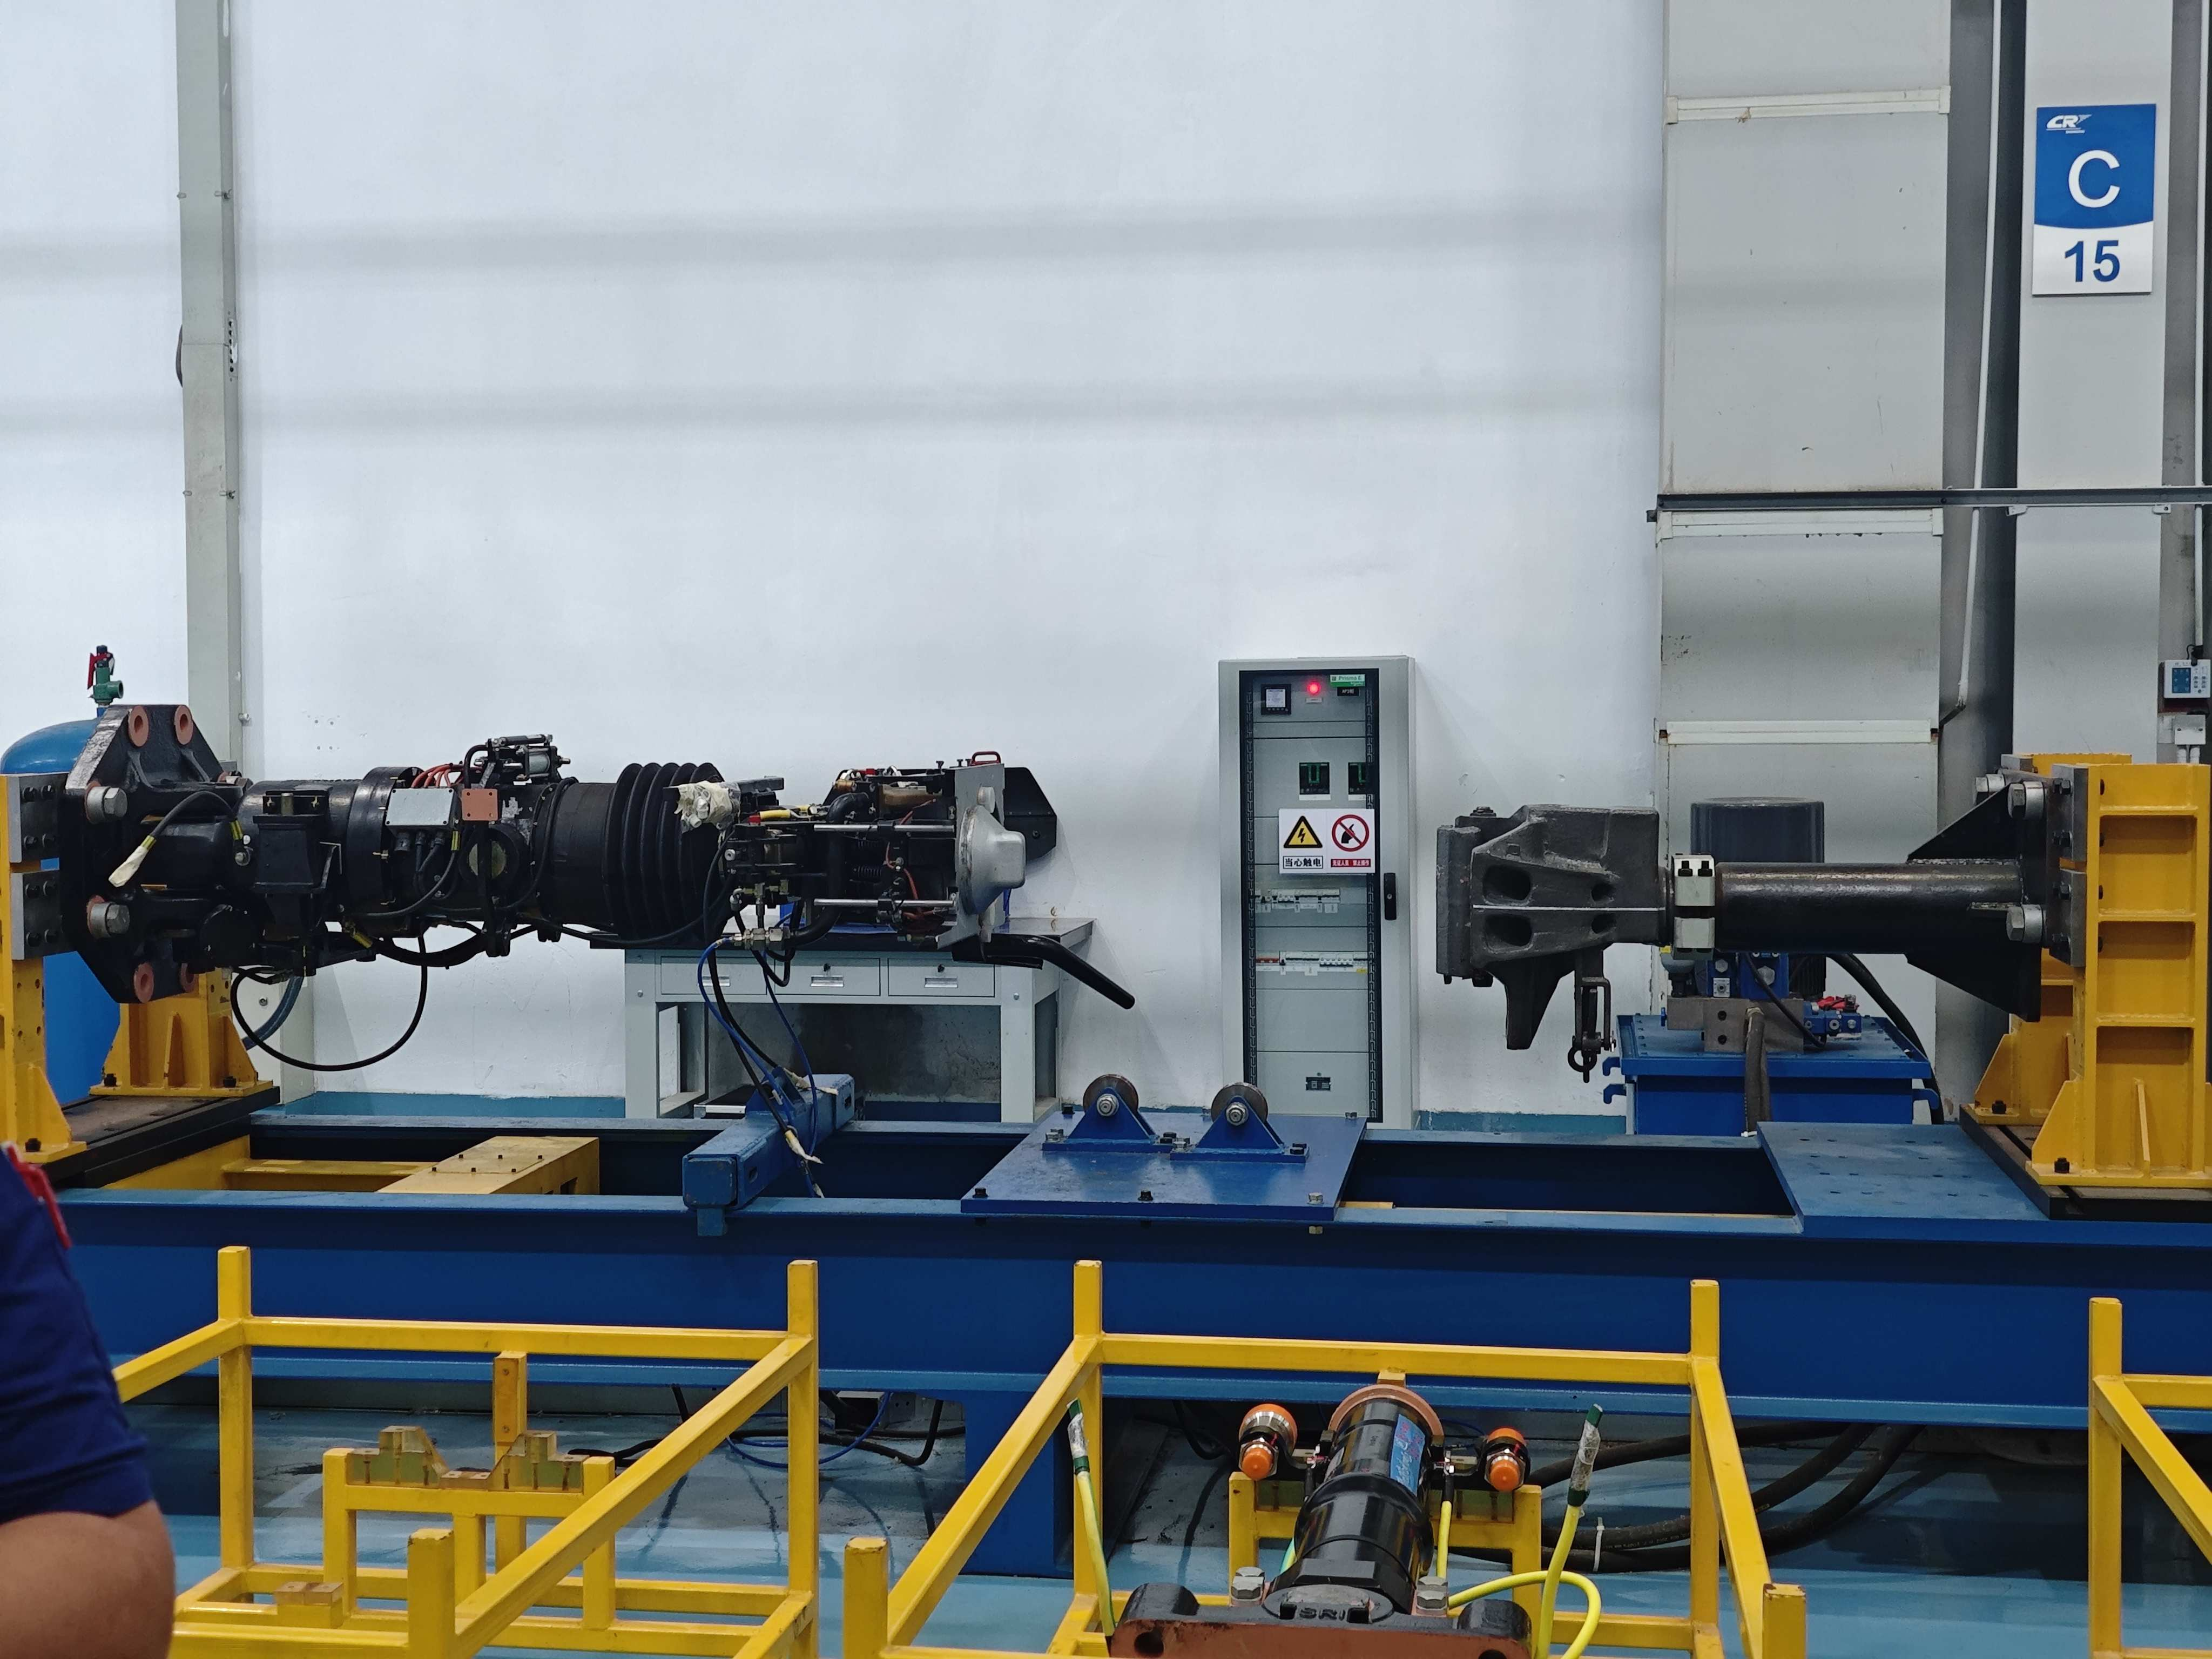
\includegraphics[width=0.32\textwidth]{assets/20260718_234802.jpg}
    \vspace{-2.5mm}
    \caption{部分工位现状}\label{fig:component-overhaul-workstations}
    \vspace{-5mm}
  \end{figure}
}

\expandafter\newcommand\csname reportFigure@16\endcsname{
  \begin{figure}[H]
    \centering
    \vspace{-1mm}
    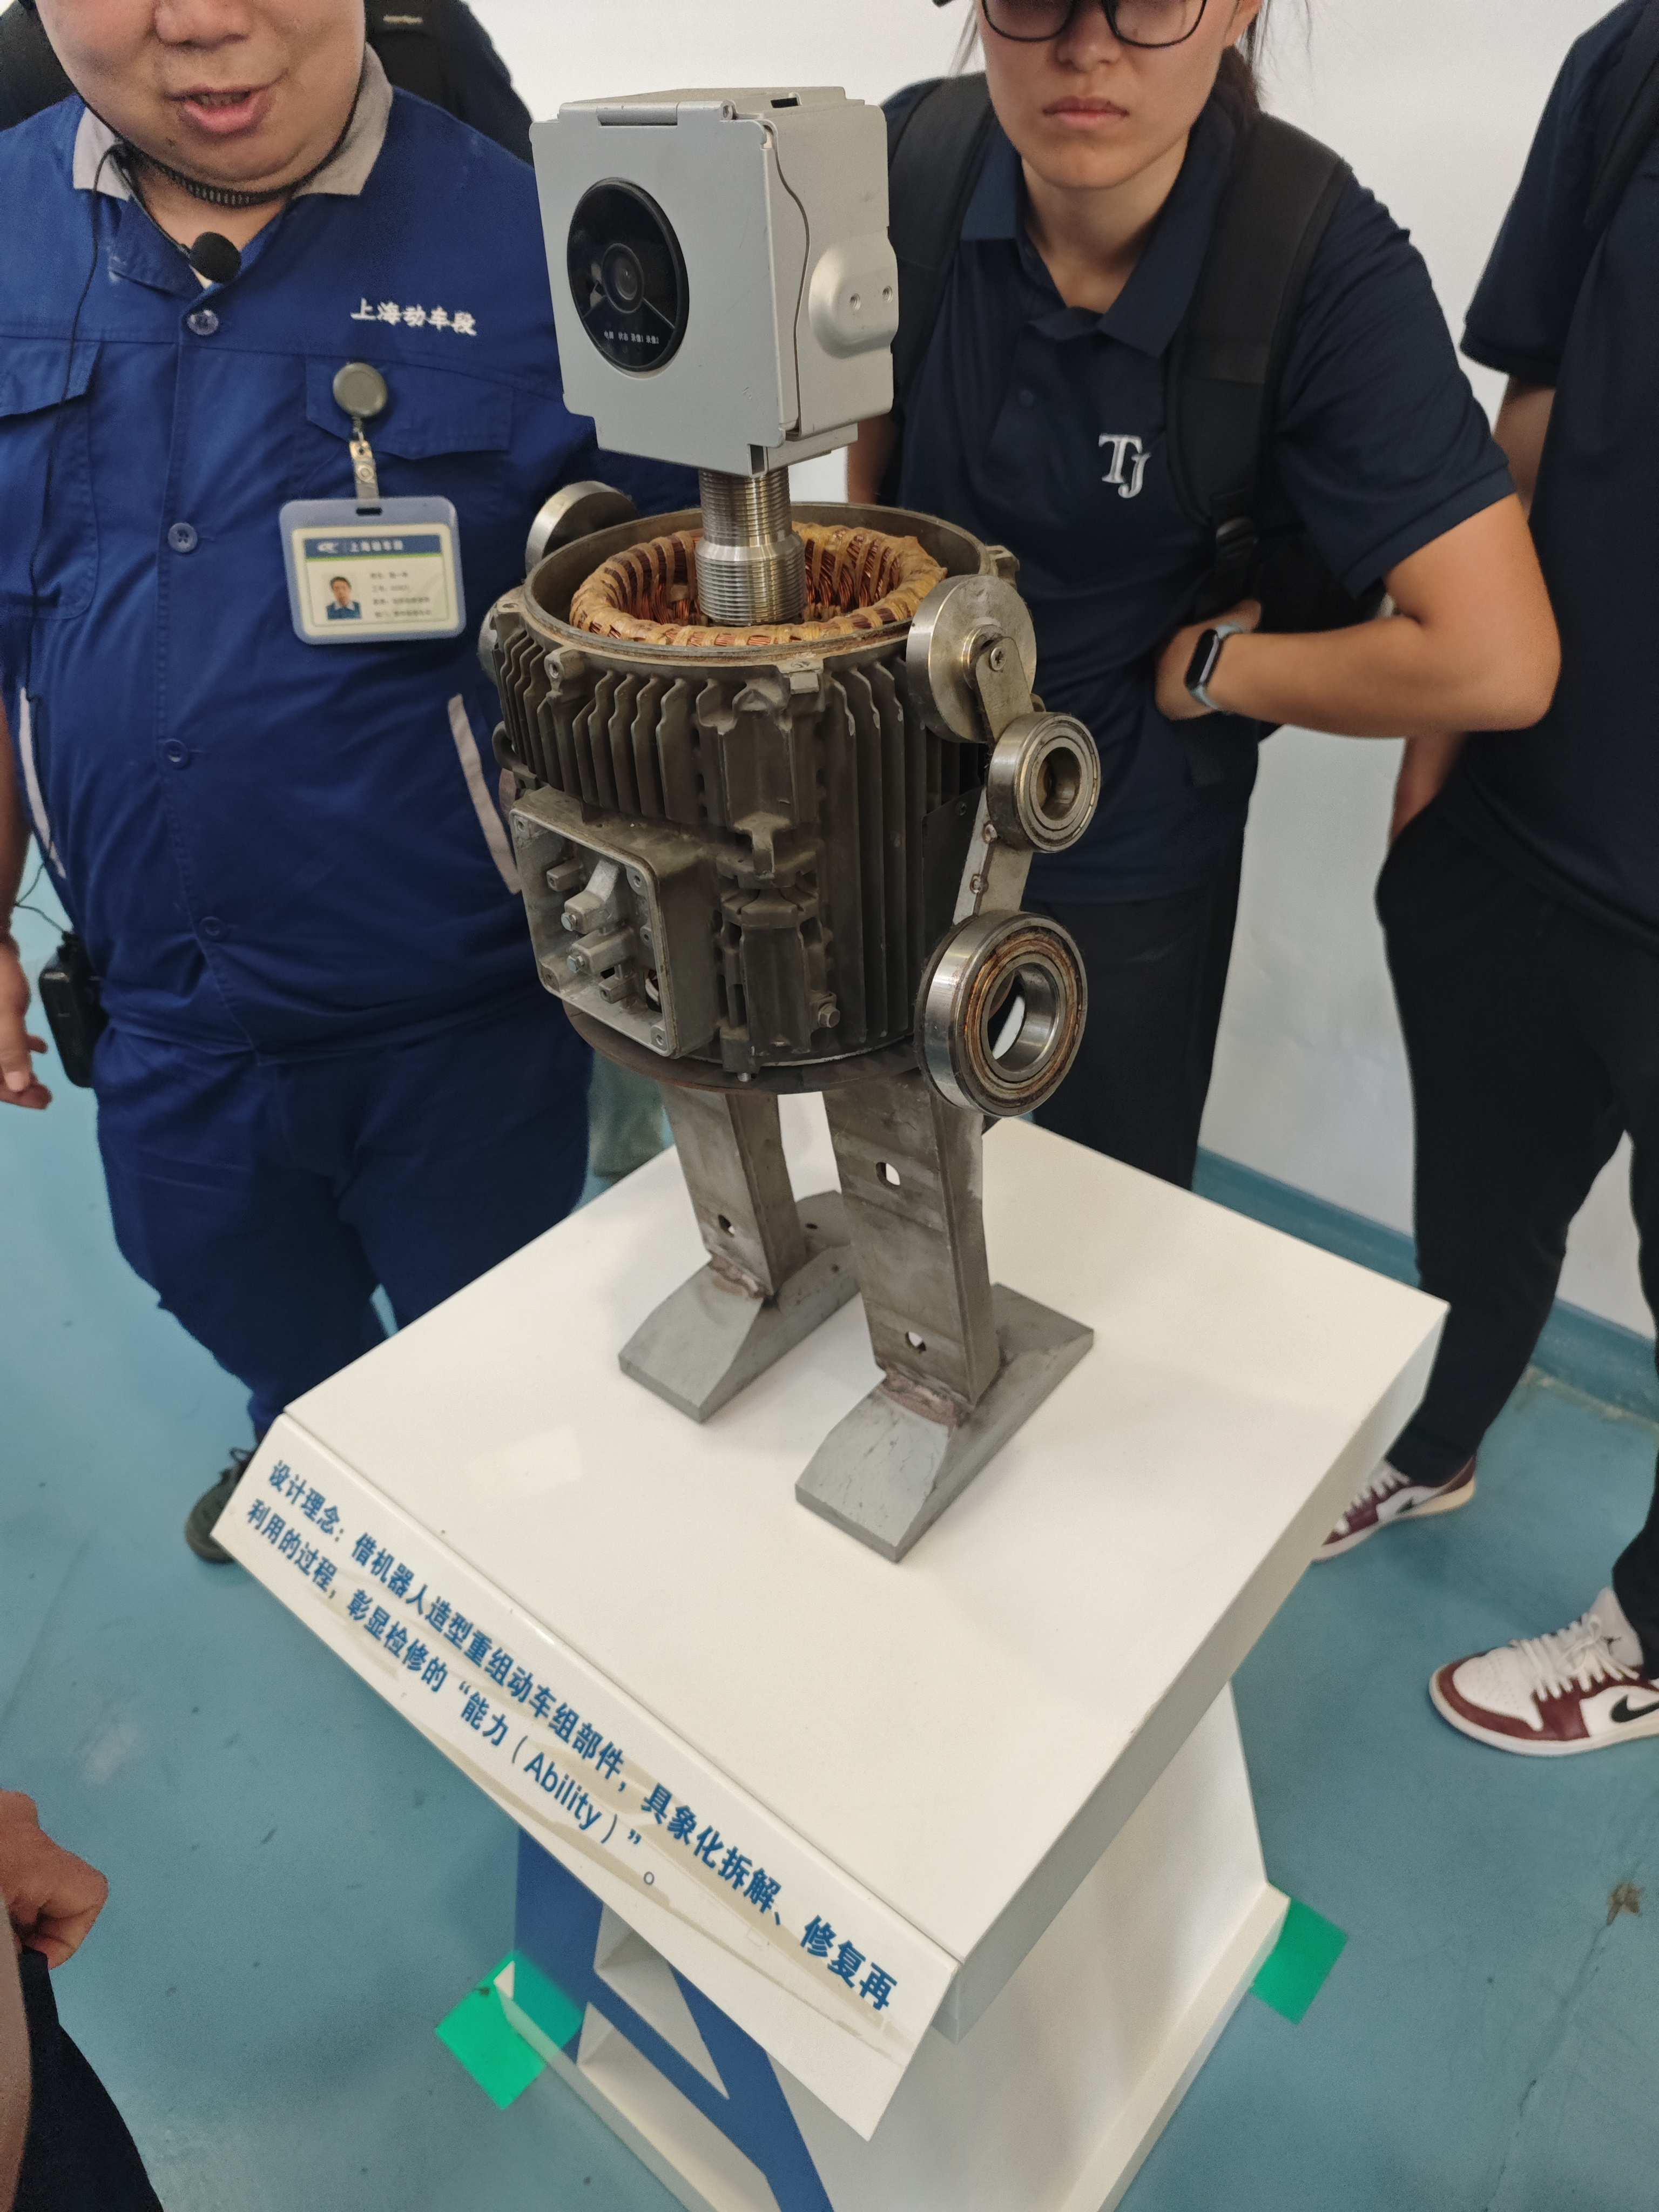
\includegraphics[width=0.5\textwidth]{assets/20260718_233942.jpg}
    \vspace{-2.5mm}
    \caption{由车上设备制作的PARTS主题艺术品}\label{fig:parts-artwork}
    \vspace{-5mm}
  \end{figure}
}

\expandafter\newcommand\csname reportFigure@6\endcsname{
  \begin{figure}[H]
    \centering
    \vspace{-3mm}
    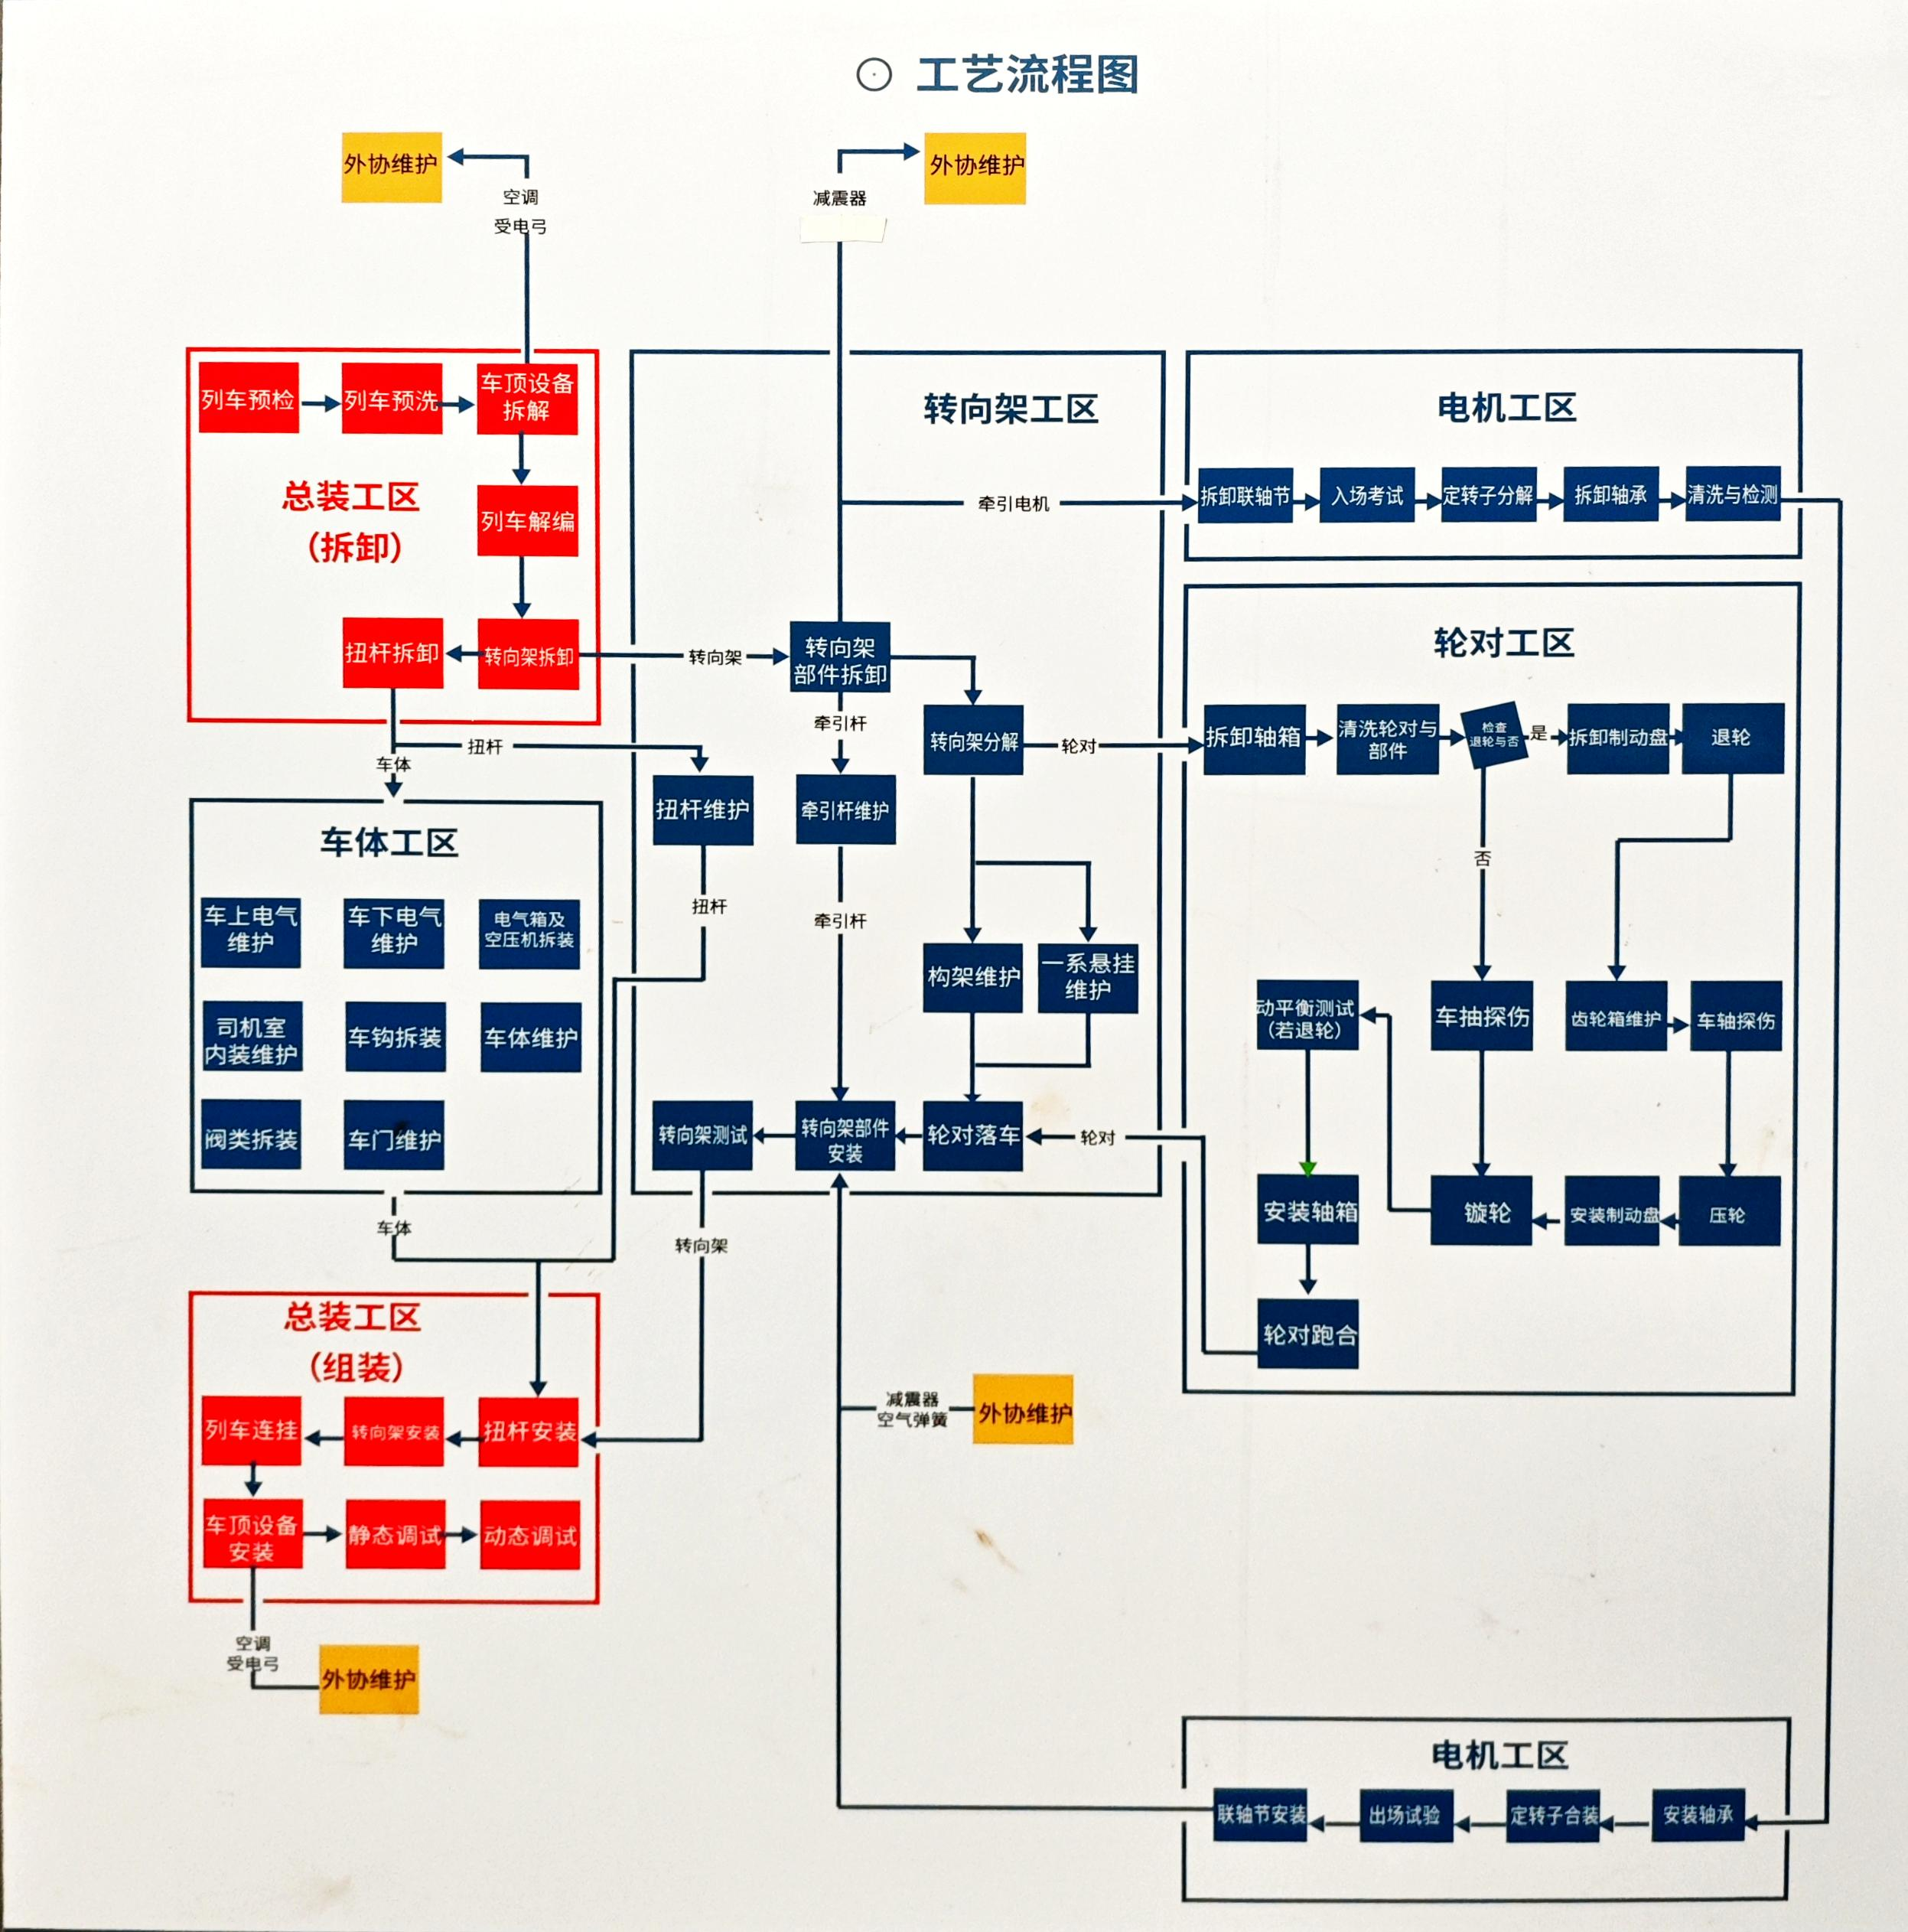
\includegraphics[width=0.98\textwidth]{assets/process-flow-corrected.jpg}
    \vspace{-2mm}
    \caption{地铁车辆检修工艺流程图}\label{fig:metro-maintenance-flow}
    \vspace{-5mm}
  \end{figure}
}

\expandafter\newcommand\csname reportFigure@7\endcsname{
  \begin{figure}[H]
    \centering
    \vspace{-3mm}
    \setlength{\tabcolsep}{1mm}
    \begin{tabular}{@{}cc@{}}
      \begin{minipage}[t]{0.48\textwidth}
        \centering
        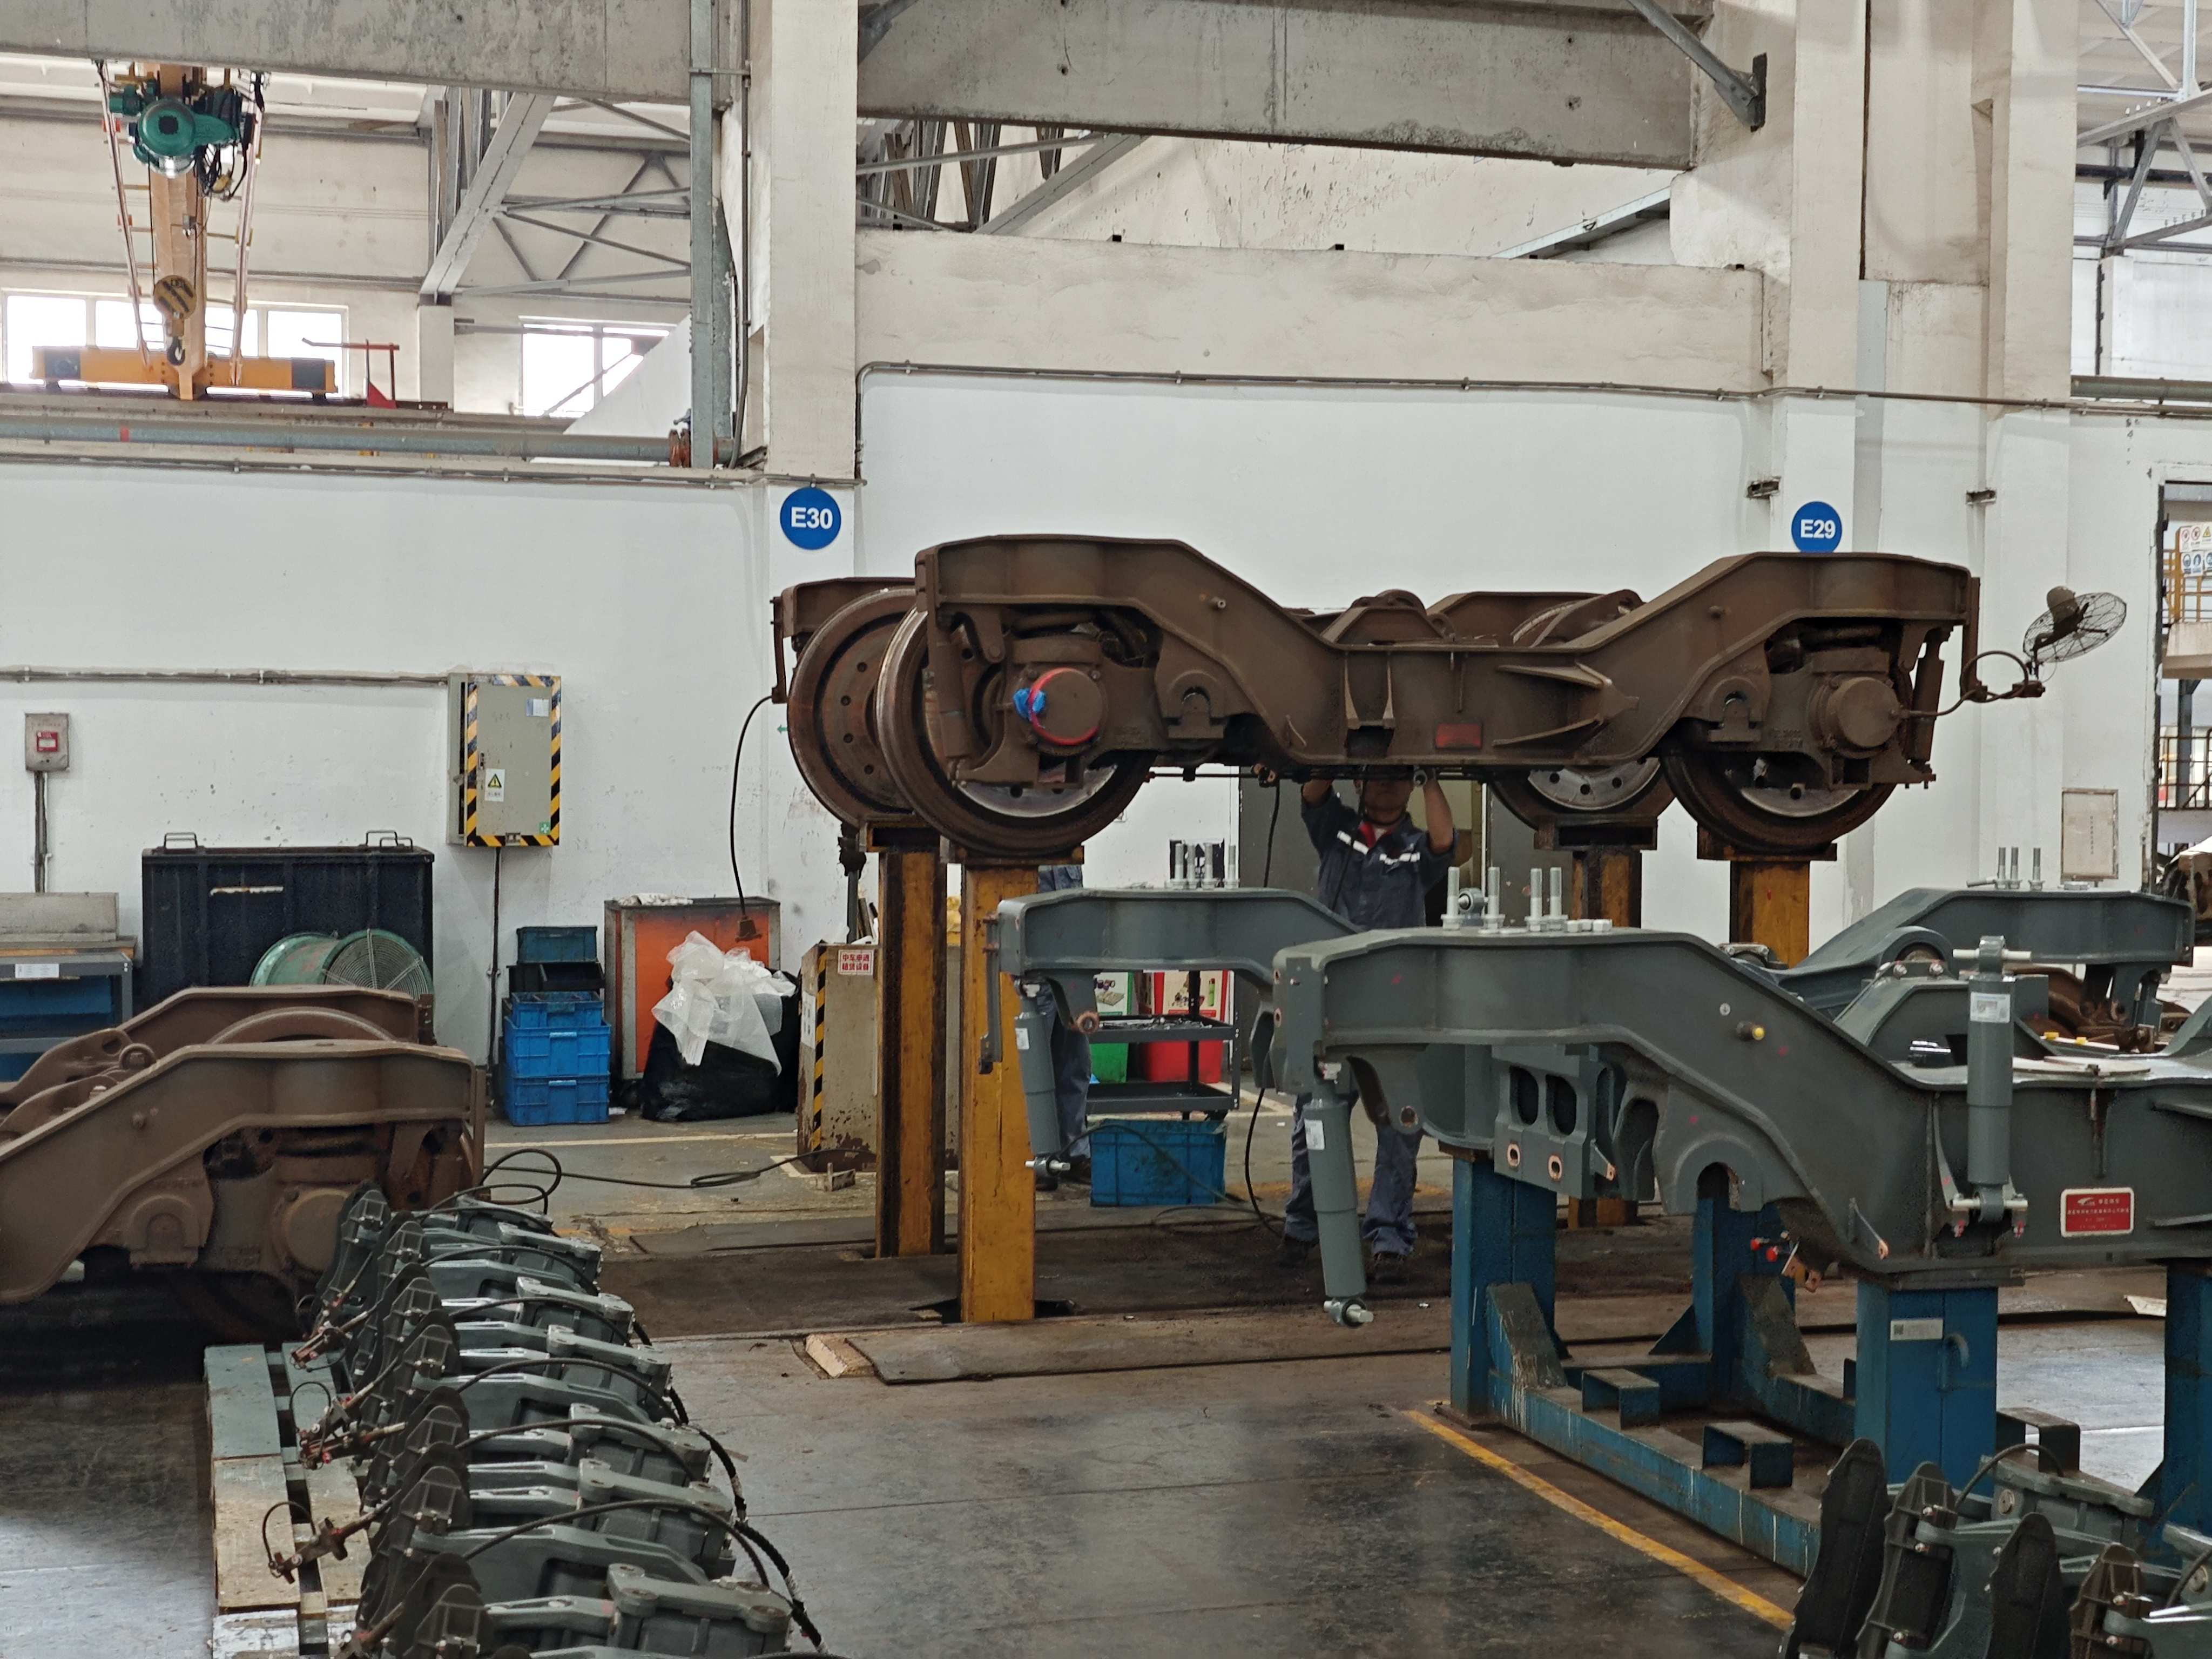
\includegraphics[height=50mm]{assets/20260717_034156.jpg}
        \par{\reportSong\fontsize{10.5pt}{12.5pt}\selectfont (a) 转向架拆卸}
      \end{minipage}
       &
      \begin{minipage}[t]{0.48\textwidth}
        \centering
        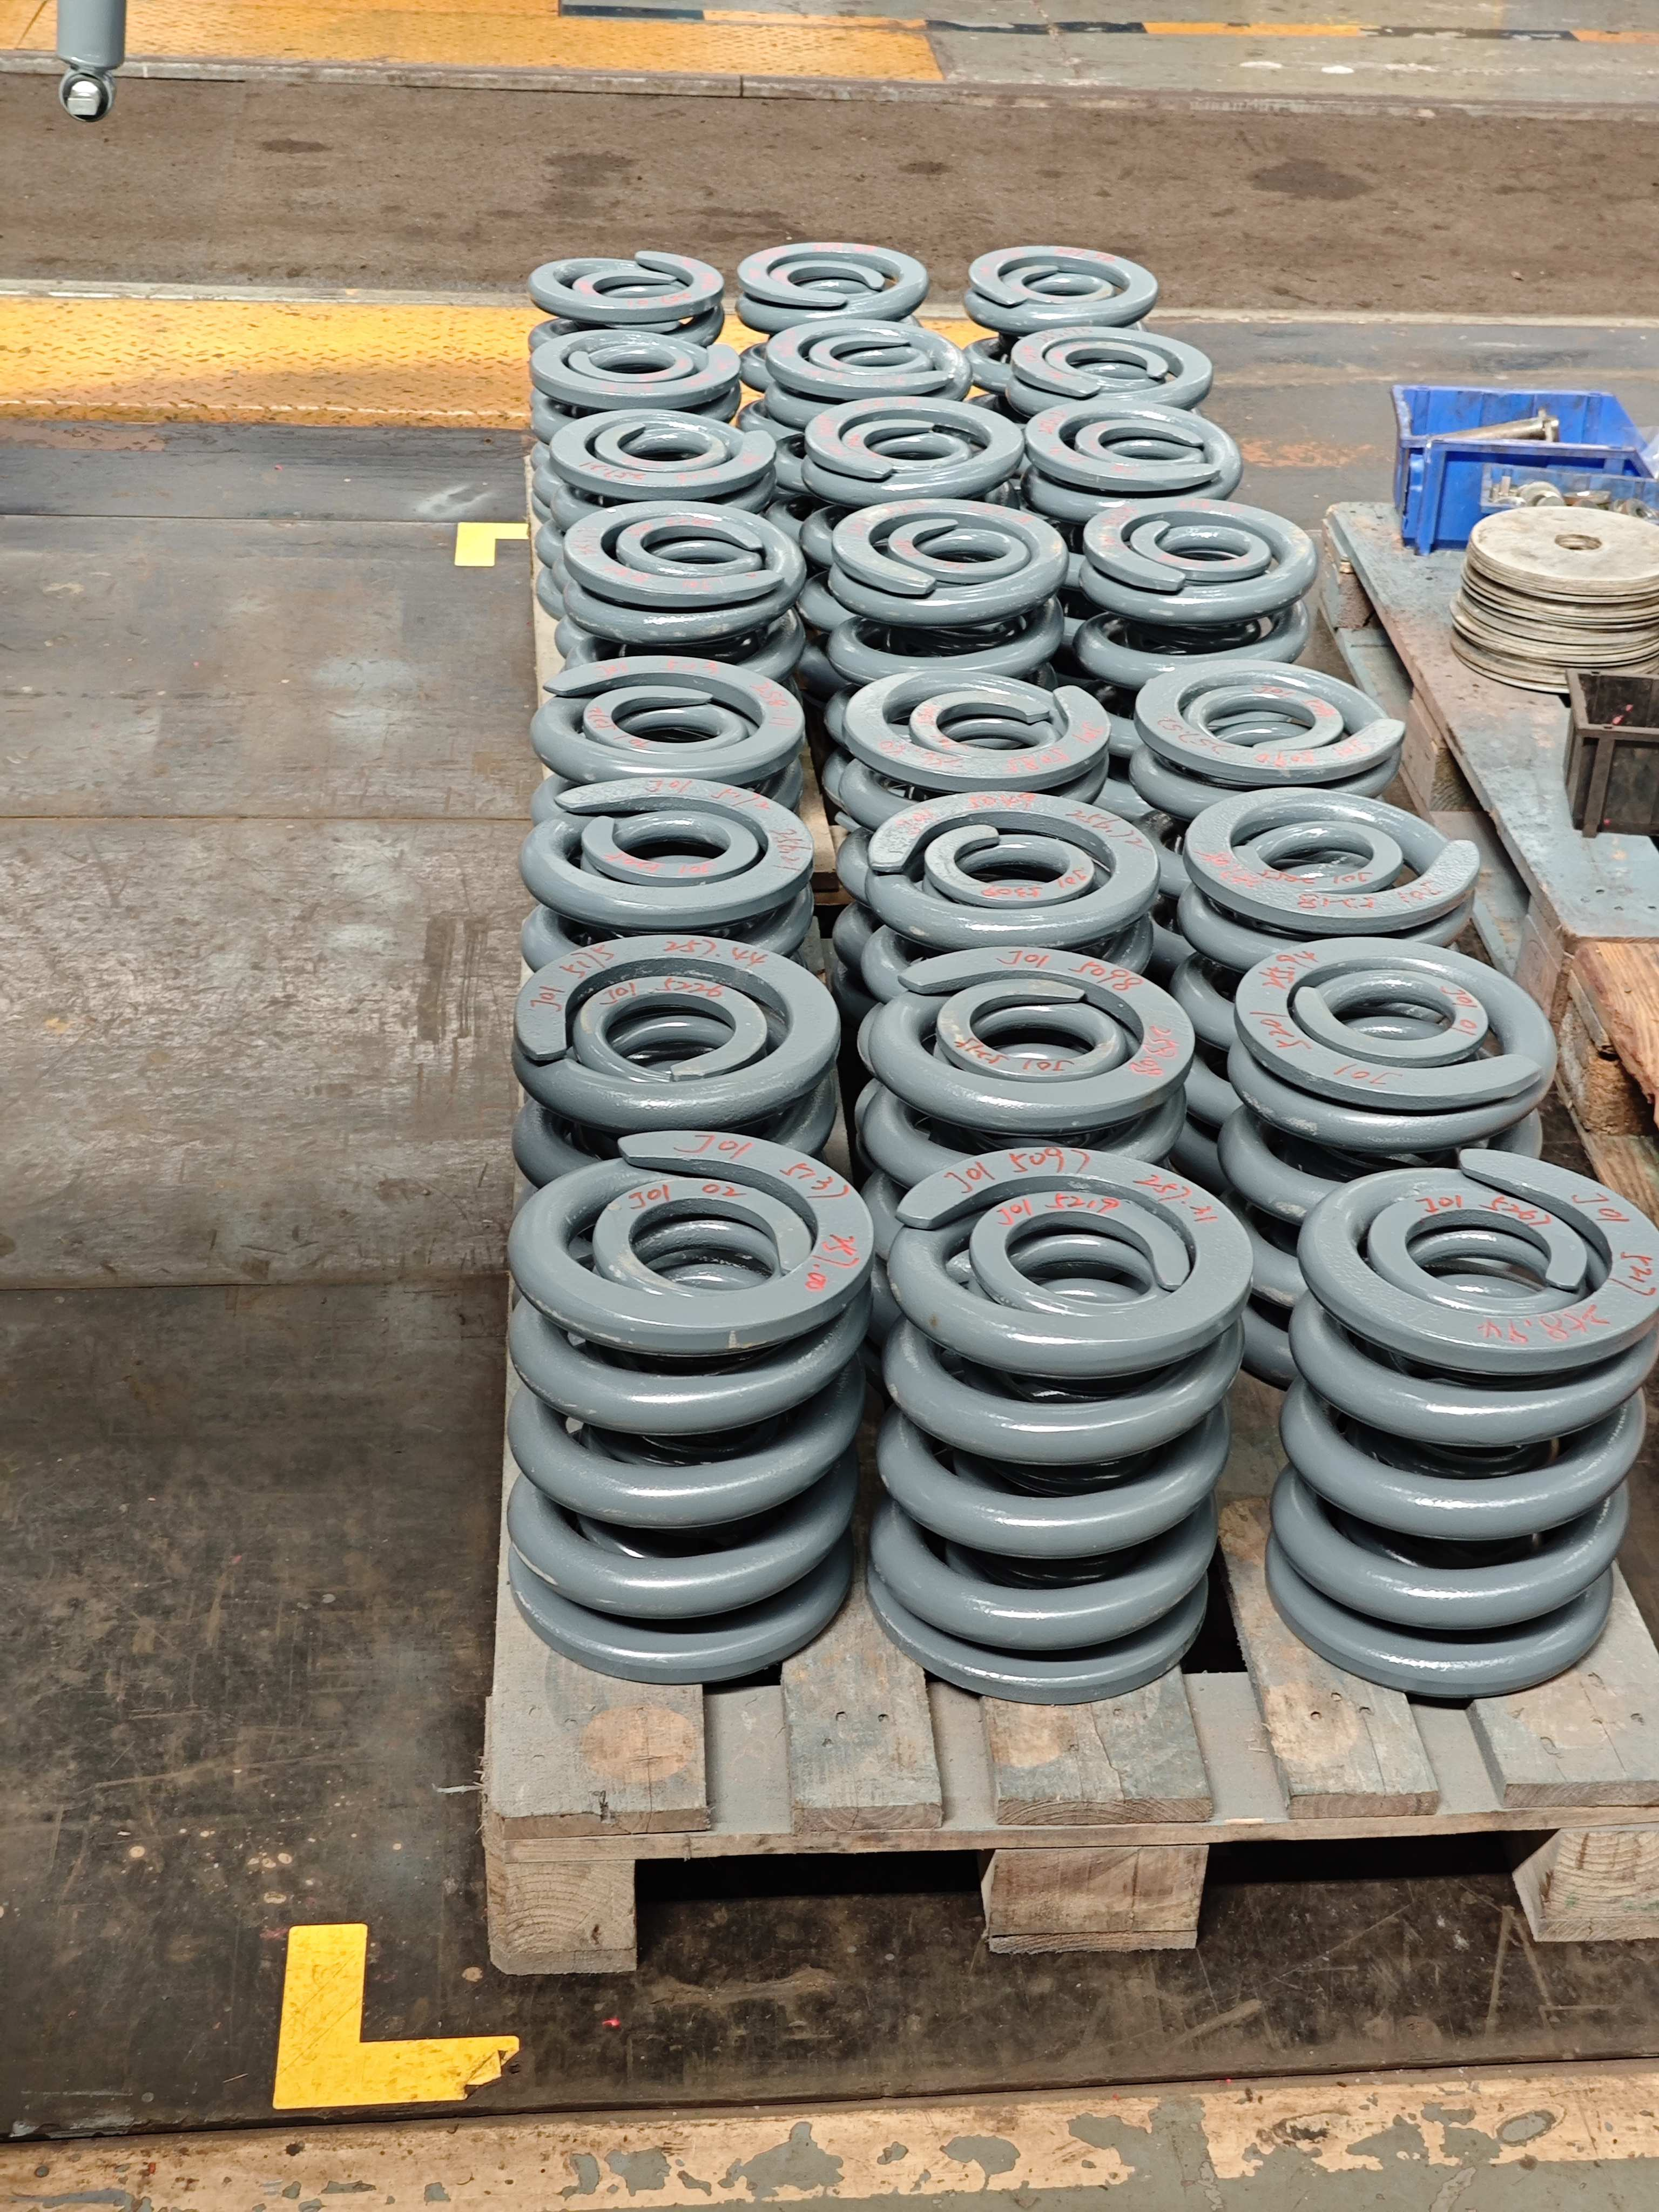
\includegraphics[height=50mm]{assets/20260717_034823.jpg}
        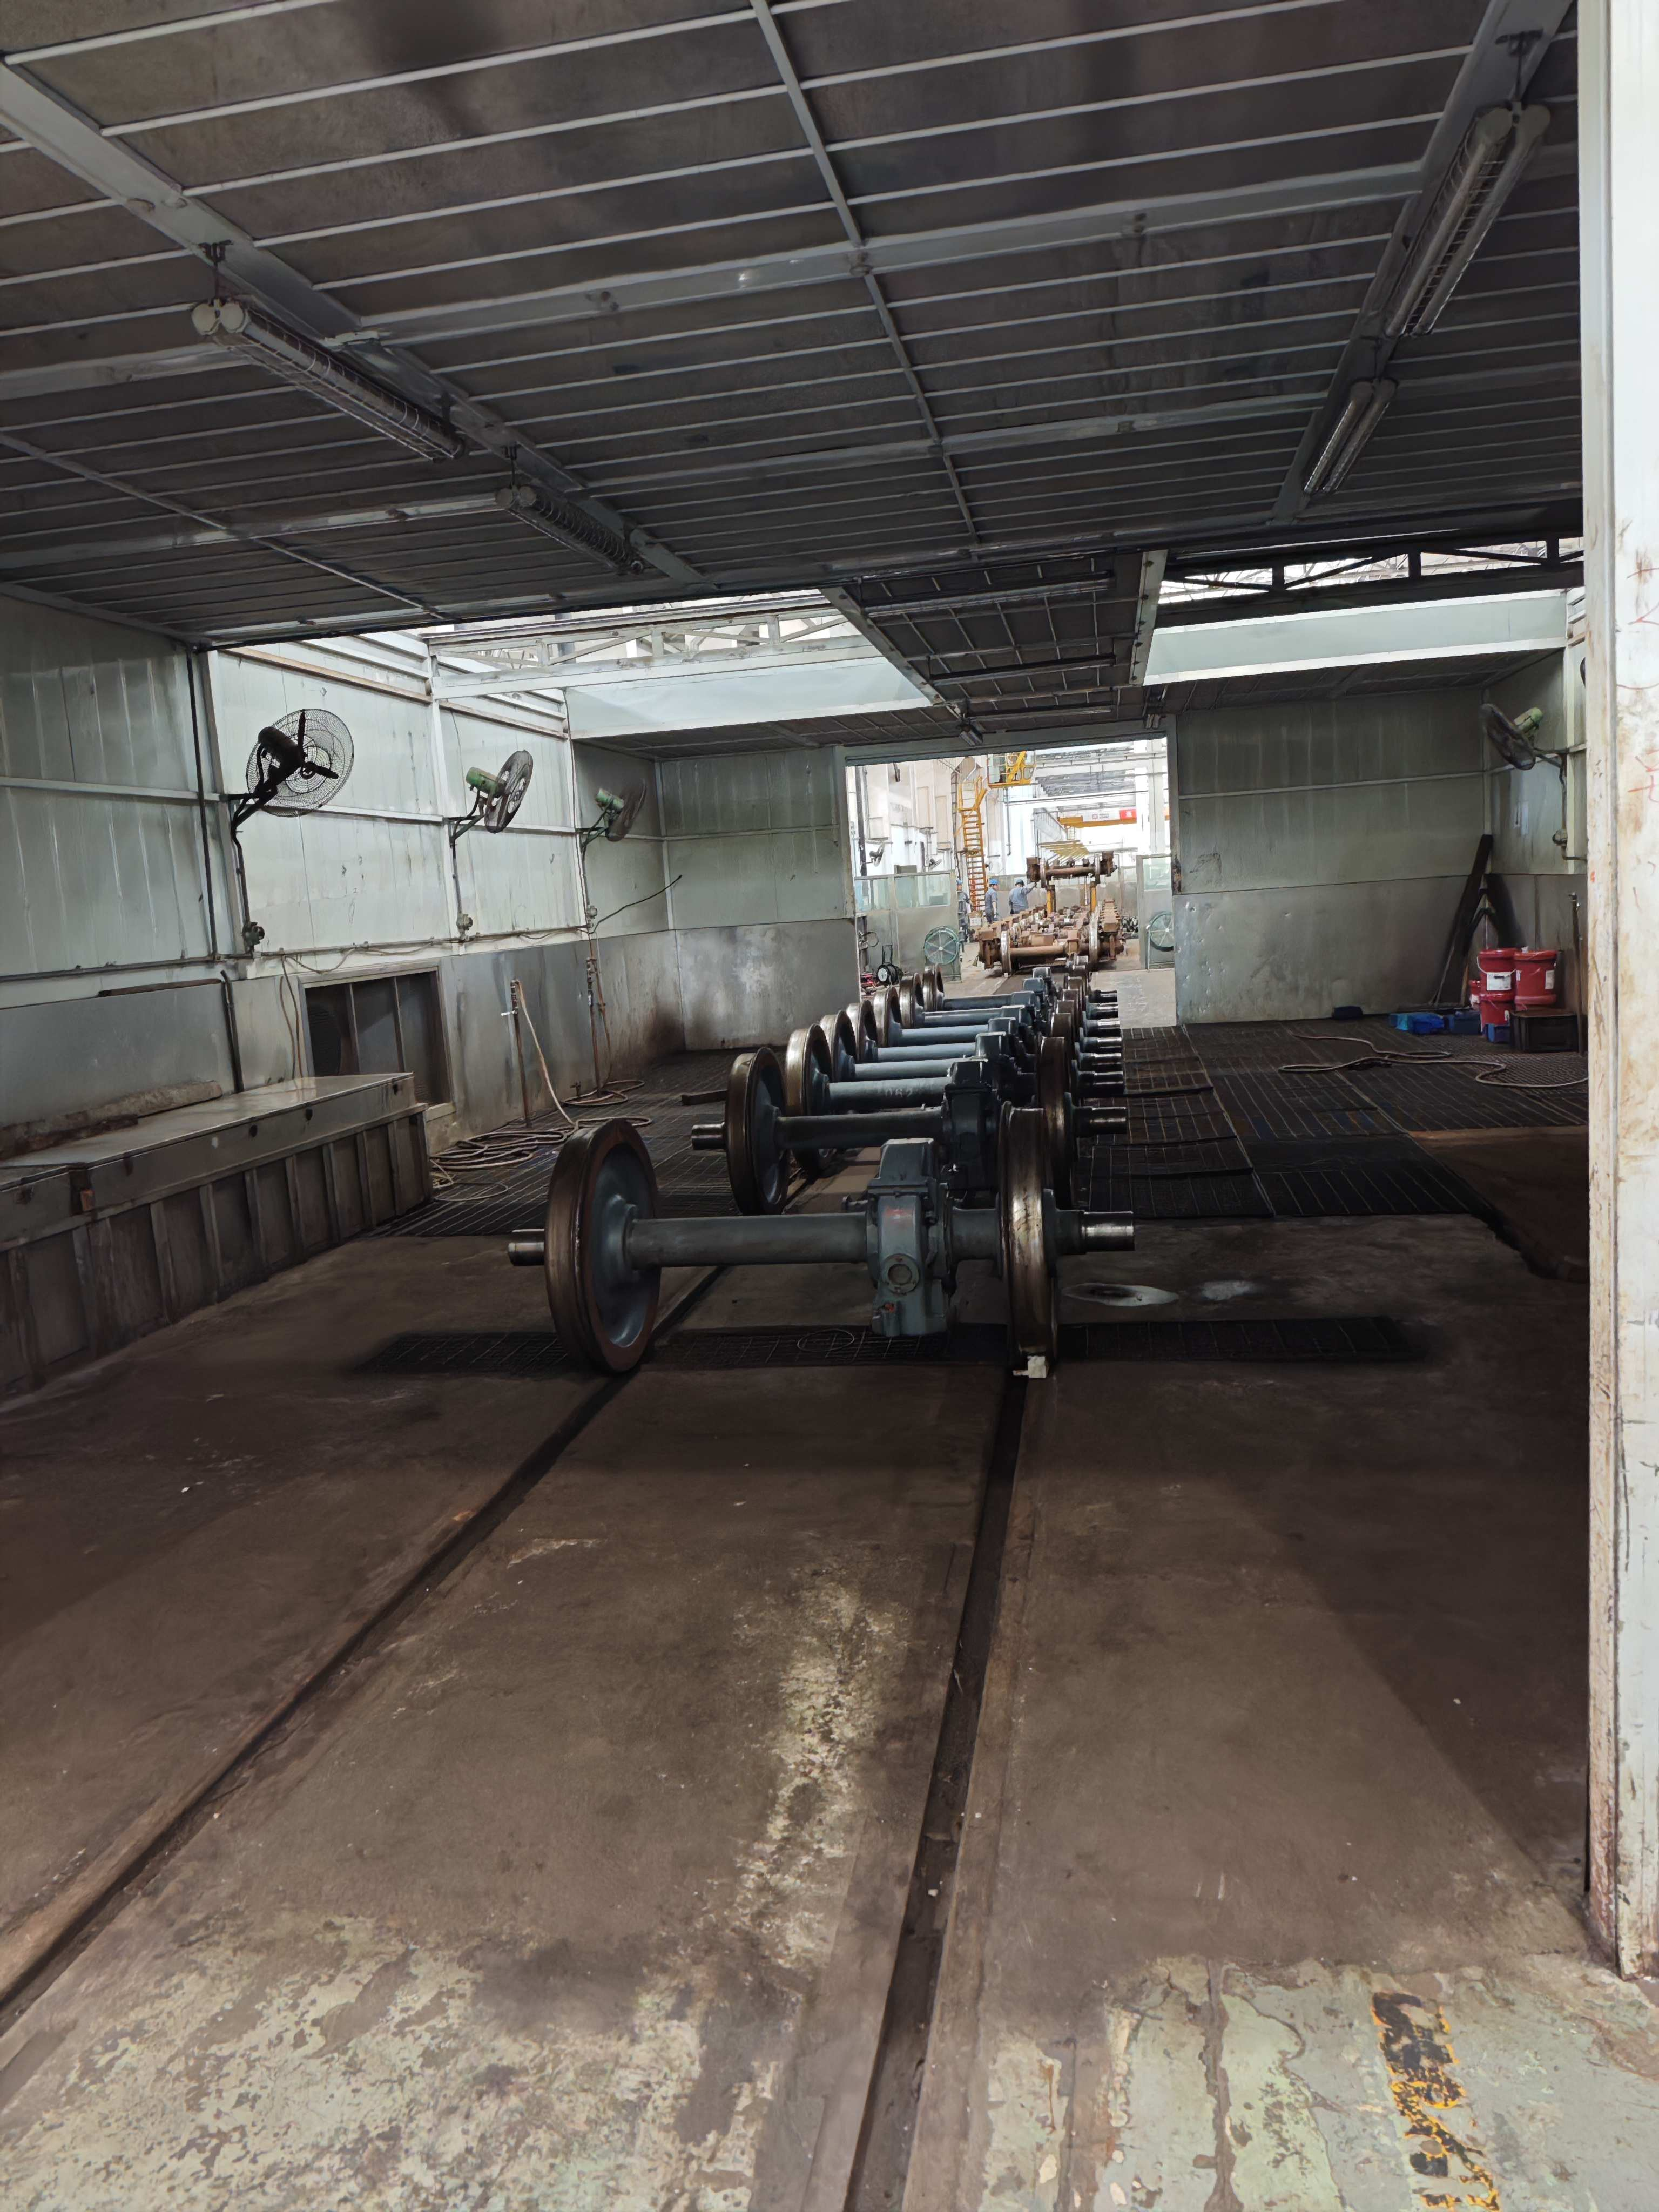
\includegraphics[height=50mm]{assets/20260717_035233.jpg}
        \par{\reportSong\fontsize{10.5pt}{12.5pt}\selectfont (b) 一系钢弹簧与轮对}
      \end{minipage}
      \\[9mm]
      \begin{minipage}[t]{0.48\textwidth}
        \centering
        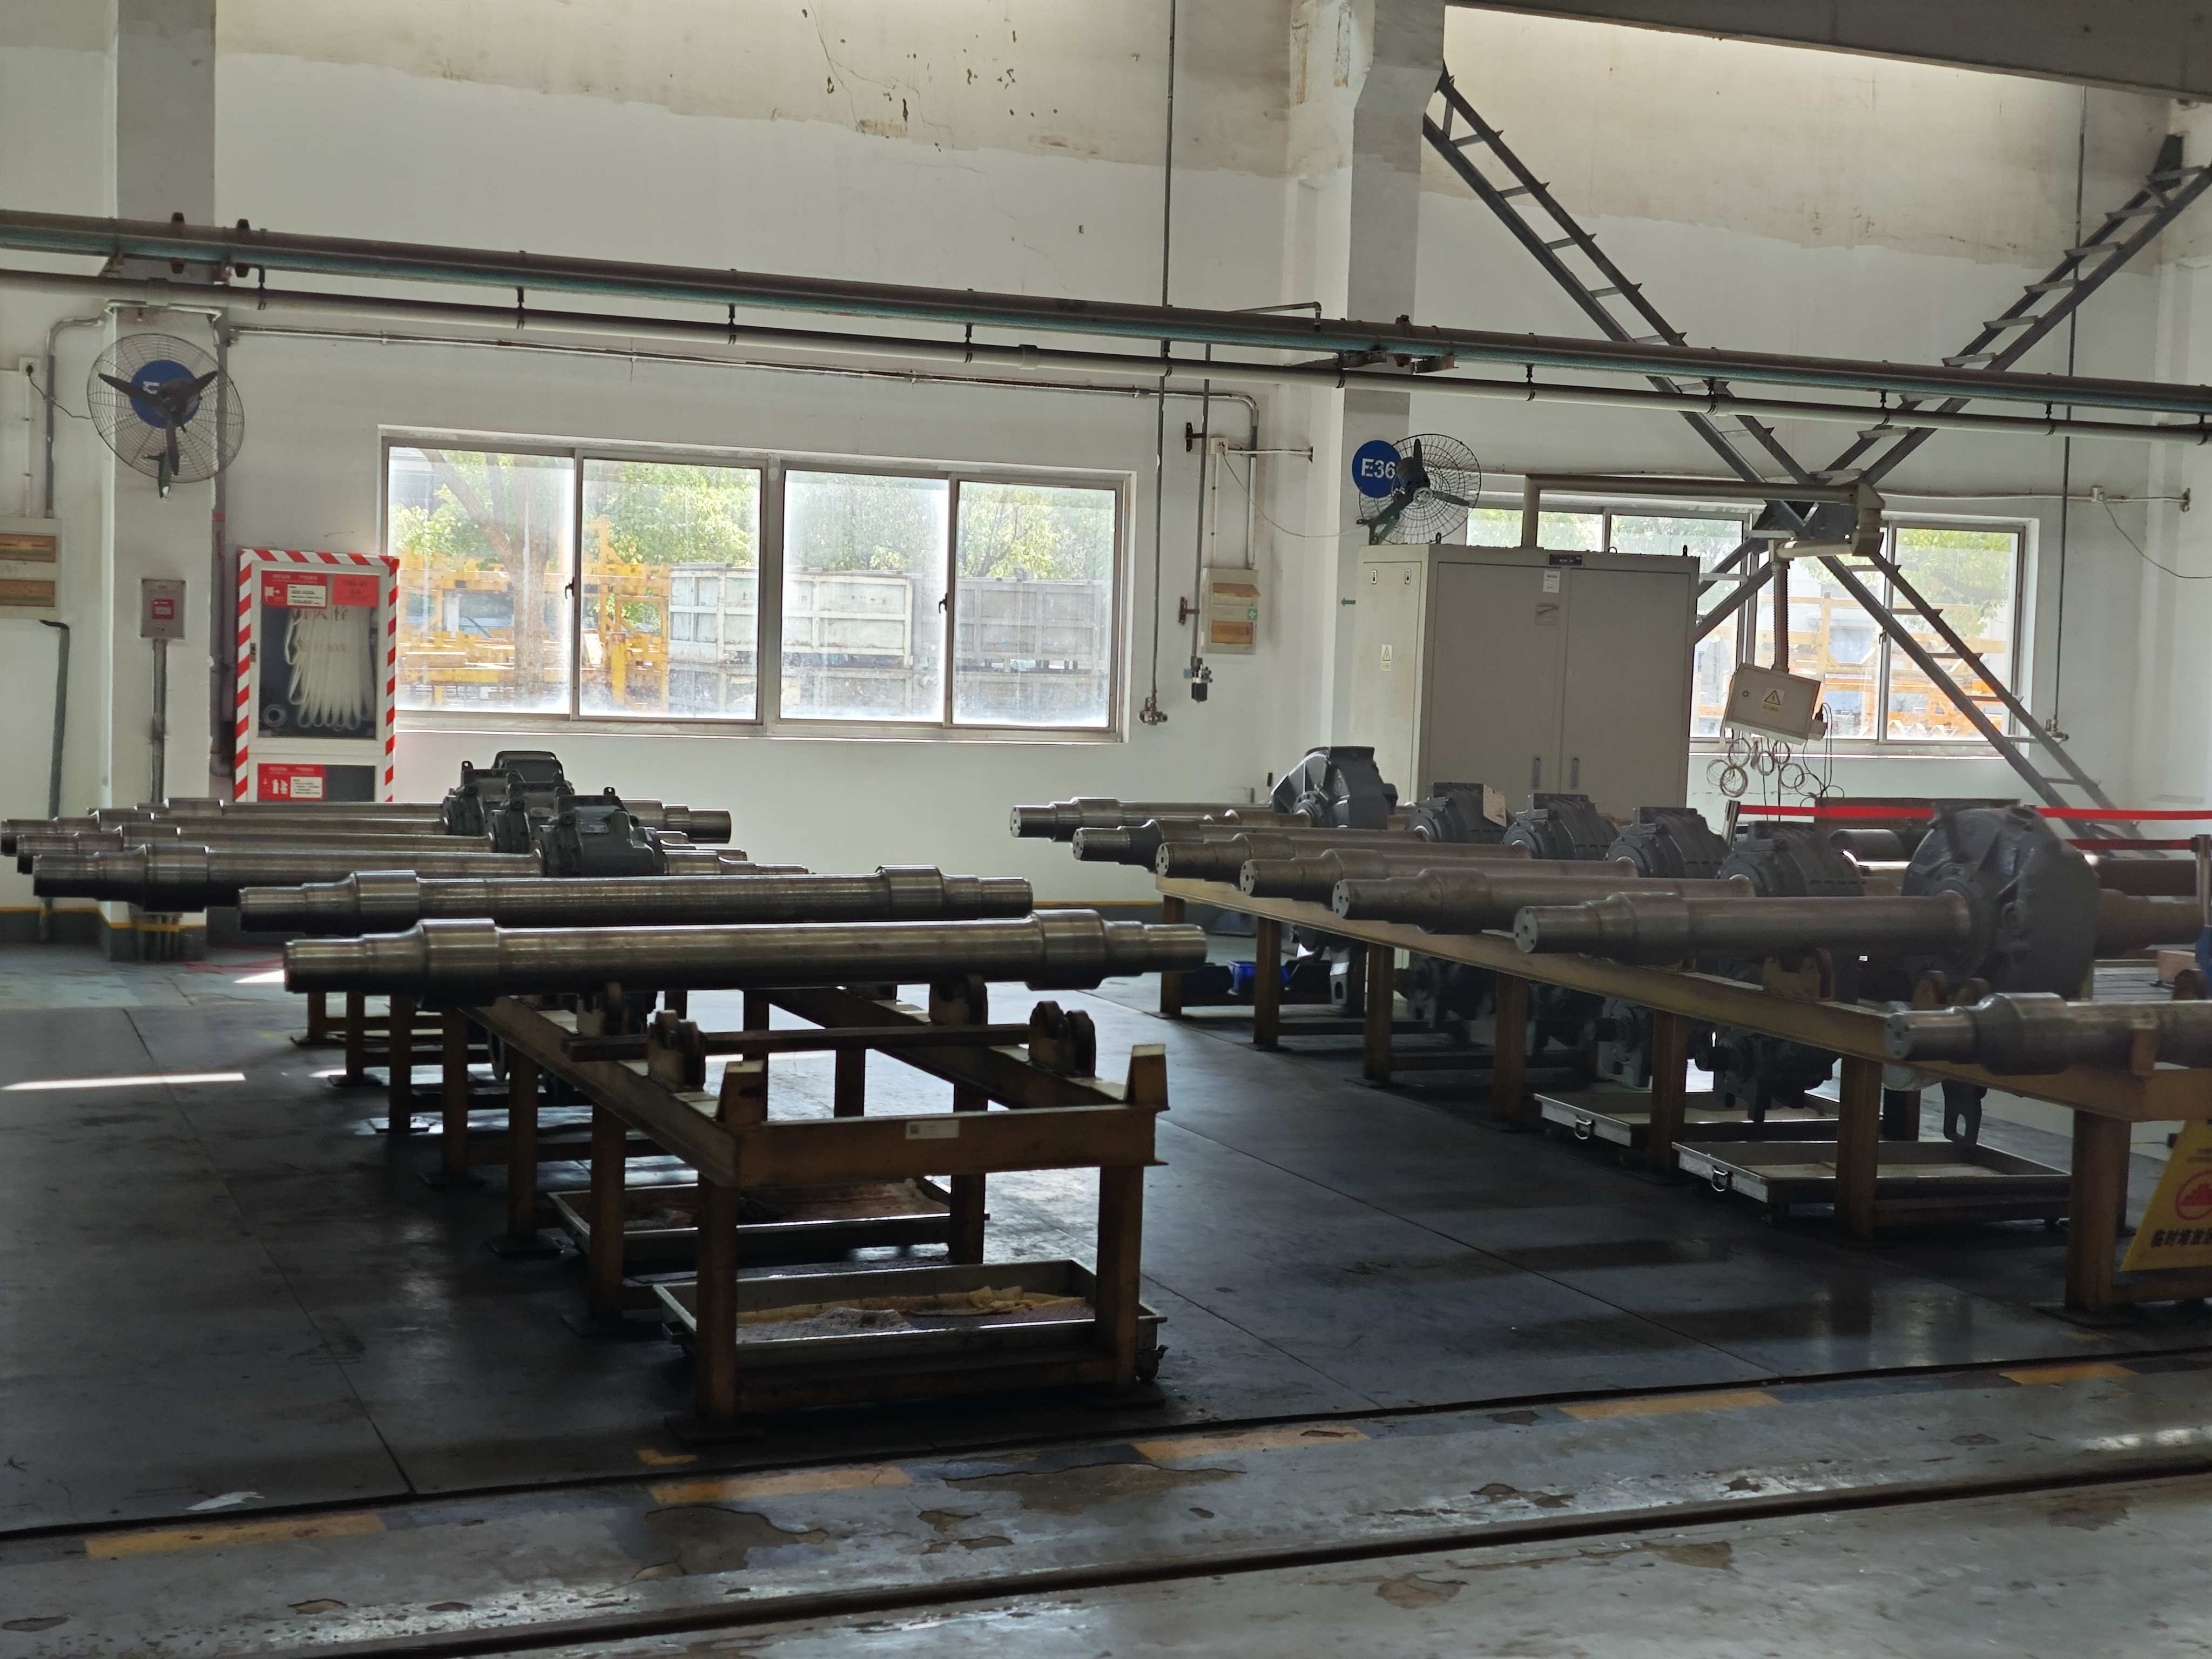
\includegraphics[height=50mm]{assets/20260717_040445.jpg}
        \par{\reportSong\fontsize{10.5pt}{12.5pt}\selectfont (c) 已卸去轮饼的车轴}
      \end{minipage}
       &
      \begin{minipage}[t]{0.48\textwidth}
        \centering
        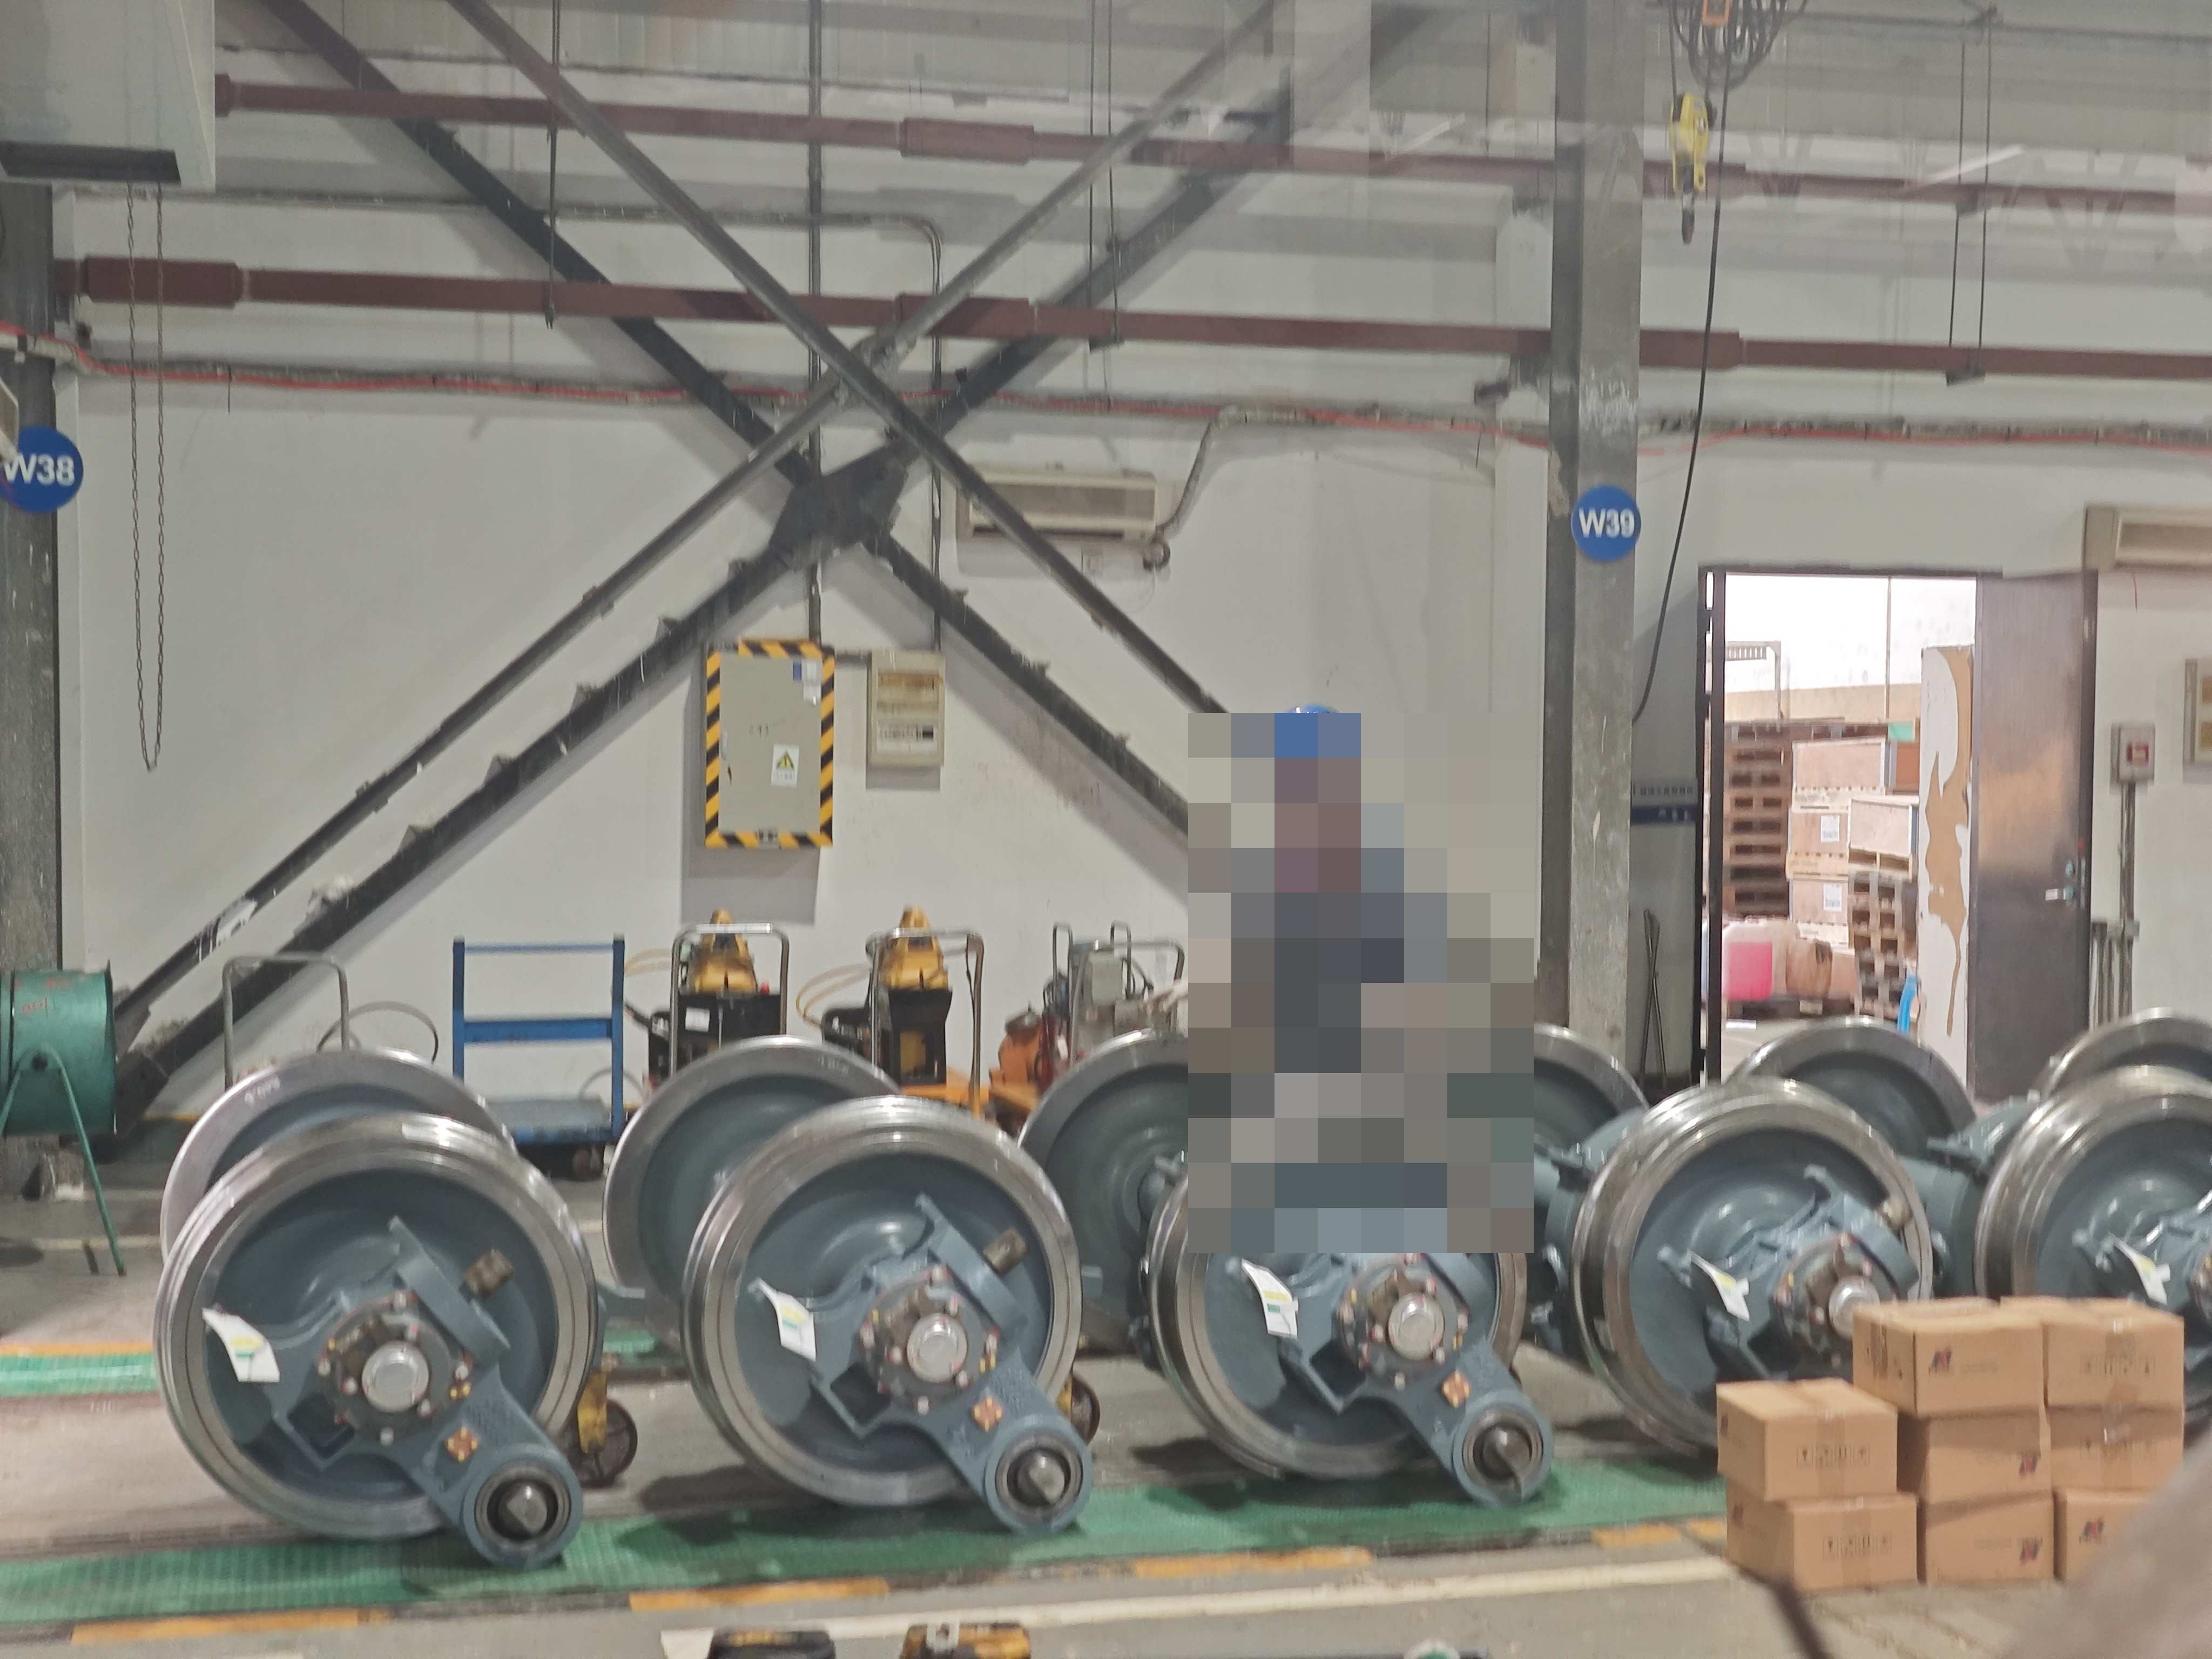
\includegraphics[height=50mm]{assets/20260717_040923_worker_mosaic_q55.jpg}
        \par{\reportSong\fontsize{10.5pt}{12.5pt}\selectfont (d) 已安装轴箱的轮对}
      \end{minipage}
    \end{tabular}
    \vspace{-2mm}
    \caption{赛车场车辆段部分检修现场}\label{fig:metro-maintenance-scenes}
    \vspace{-5mm}
  \end{figure}
}
